%-----------------------------------------------------------------------
% Latex Thesis/Dissertation Template for Wright State University
% 
% Written by Sean A. Mortara
% 28 June 2001
% Modified by Josh Mark
% 15 Dec 2011
% Later edits by Joseph C. Slater
%-----------------------------------------------------------------------
\documentclass[12pt]{report}

\usepackage{xcolor}
\usepackage{booktabs} % used for tables
\usepackage{multirow} % used for tables to merge multiple rows
\usepackage{bigdelim} % used for tables to set spacing
\usepackage{bigstrut} % used for tables to set spacing
\usepackage{graphicx} % used for includegraphics

\usepackage{subfigure} % allows the use of subfigures
\usepackage{amssymb,amsmath} % For math
\usepackage{graphicx, float, subfigure, caption} % For figures
\usepackage[framed,numbered,autolinebreaks,useliterate]{mcode} % used to insert code
%
\usepackage[hidelinks]{hyperref}
\usepackage{xcolor}
\hypersetup{
    colorlinks,
    linkcolor={blue!50!black},
    citecolor={blue!50!black},
    urlcolor={blue!80!black}
}
%-----------------------------------------------------------------------
%  Modified fields
%-----------------------------------------------------------------------
\newcommand{\authorfirst}{Koorosh}
\newcommand{\authorMI}{}
\newcommand{\authorlast}{Gobal}
\newcommand{\degreefull}{Doctor of Philosophy}  % force hyphenation at syllables if line breaks are required
\newcommand{\degreeshort}{Ph.D.}
\newcommand{\thesisordissertationlc}{Dissertation}
\newcommand{\dept}{Department of Mechanical Engineering}
\newcommand{\institution}{Wright State University} % Doubting you will
                                % change this. 
\newcommand{\thesistitle}{High-Fidelity Multidisciplinary Sensitivity Analysis for Coupled Fluid-Solid Interaction Design} % Needes a line break
\newcommand{\bachdegreeshort}{B.S.M.E.} % Bachelor degree short
\newcommand{\bachinstitution}{Sharif University of Technology} % Bachelor degree institution
\newcommand{\bachyear}{2012}% Bachelor degree year
%No spaces should be before or after this title.
\newcommand{\pdfsubject}{Shape Sensitivity Analysis for FSI Design}
\newcommand{\pdfkeywords}{Sensitivity Analysis, Fluid-Solid Interaction, Multidisciplinary Design Optimization}
\newcommand{\yearcomplete}{2016}
% set pdf file info
\usepackage{hyperxmp} % used to set pdf property info with \hypersetup command

%-----------------------------------------------------------------------
%  Thesis Advisor, Department Chair, Dean of Graduate Studies
%  I don't know why titles as separated... except in the one case at
%  the end. 
%-----------------------------------------------------------------------
\newcommand{\thesisdirector}{Ramana V. Grandhi}
\newcommand{\thesisdirectortitle}{Ph.D.}
\newcommand{\phdProgrameChair}{Frank W. Ciarallo}
\newcommand{\phdProgrameChairTitle}{Ph.D.}
\newcommand{\graduateSchoolDean}{Robert E.W. Fyffe}
\newcommand{\graduateSchoolDeanEducation}{Ph.D.}
\newcommand{\graduateSchoolDeanTitle}{Vice President for Research and \\Dean of the Graduate School}
%-----------------------------------------------------------------------
%  Final Examination Committee: Comment out the ones you don't need. 
%-----------------------------------------------------------------------
\newcommand{\fecone}{Ramana V. Grandhi, Ph.D.}

\newcommand{\fectwo}{Mitch Wolff, Ph.D.}

\newcommand{\fecthree}{Ha-Rok Bae, Ph.D.}

\newcommand{\fecfour}{Robert A. Canfield, Ph.D.}

\newcommand{\fecfive}{Raymond M. Kolonay, Ph.D.}

\newcommand{\fecsix}{Christopher M. Koehler, Ph.D.}

% If you have more committee members... good luck

% Modify this if needed for getting citations to "look right" according to your field. Read the natbib documentation on how to use this. 
%\usepackage[round]{natbib}
%\usepackage{doublespace}

%=============================
%  Begin document!
%=============================
%
% Don't touch

% still don't touch.   

% title sheet
\usepackage{WSU}
%\hypersetup{
%                     pdfauthor={\authorfull},
%                     pdftitle={\thesistitle},
%                     pdfsubject={\pdfsubject},
%                     pdfkeywords={\pdfkeywords},
%                     }
% \normalem
\pagenumbering{roman}
\pagestyle{plain}
\rhead{October 5, 2016}
\begin{document}
\maketitle
\doublespace

% Still don't touch!!

%=============================
%  approval sheet
%=============================

\thispagestyle{empty}
\renewcommand\baselinestretch{2}
\begin{singlespace}
\signaturepage
\end{singlespace}
%
%=============================
%  Abstract
%=============================
\newpage
\setcounter{page}{3}
\vspace{2in}
%
\begin{singlespace}
\begin{center}
  ABSTRACT
\end{center}
%
\noindent{\small{\authorlast, \authorfirst}. 
		 {\degreeshort, Engineering Ph.D. Program, \dept, \institution}, 
		 {\yearcomplete}. 
		 {\thesistitle}.}
\end{singlespace}
\vspace*{.5in}

\pdfbookmark[0]{Abstract}{Abstract}
%\phantomsection
%
%========================
% Start editing below. 
%========================
In many engineering disciplines such as aerospace, marine, automotive, and biomedical engineering the consideration of the coupling between the fluid and structural systems is necessary for quality engineering analysis. Therefore, the need for such analysis in the design is continuously increasing. The primary motivation for this work is to develop a sensitivity analysis tool that is capable of calculating accurate sensitivities without significant modification of the source codes for simulations based on non-body conformal grids. The majority of work done on the coupled fluid-solid simulations are based on computational grids that conform to the solid boundaries. This becomes a restriction for complex boundary shapes or large deformation of the solid domain. The hurdles associated with the body-conformal techniques are mainly due to additional cost related to mesh deformation and the effect of mesh movement on the sensitivity calculation. Therefore, we propose to use a particular family of non-body conformal techniques often known as Immersed Boundary (IB) methods for modeling the flow over immersed boundaries. The Continuum Sensitivity Analysis (CSA) is added on top of the IB method, which calculates the sensitivity of the flow variables, velocity, and pressure. These variables are modeled with Navier-Stokes (NS) equations and their sensitivities are calculated with respect to change in the shape of the solid boundary. This technique is implemented in the calculation of the sensitivity of the coupled fluid-structure system subject to different shape design variables. The sensitivity of various benchmark problems such as flow between parallel plates, over a cylinder, and through a convergent-divergent nozzle is calculated with respect to shape parameters using this approach. These results are verified using the complex step method which gives accurate sensitivities up to machine precision. This work is the first implementation of CSA for continuous IB method for viscous flow (Navier-Stokes) models.

%%%%%%%%%%%%%%%%%%
%-----------------------------------------------------------------------
%
%=============================
%  List of symbols (Optional)
%=============================
%\newpage
%%\renewcommand\baselinestretch{1.5}
%\begin{singlespace}\begin{center}
%  \textbf{\Huge{List of Symbols}}
%\end{center}
%
%\begin{flushleft}{\large Chapter 2} \end{flushleft}
%\begin{tabular}{p{0.75in}l}
%   $\gamma$ & $\frac{-b+\sqrt{b^{2}-4ac}}{2a}$\\
%   $L$ & {Plate length}\\
%\end{tabular}
%
%%%%%%
%\begin{flushleft}{\large Chapter 3} \end{flushleft}
%\begin{tabular}{p{0.75in}l}
%   $h$ & {Plate thickness}\\
%   $L$ & {Plate length}\\
%\end{tabular}
%
%%%%%%
%\begin{flushleft}{\large Chapter 4} \end{flushleft}
%\begin{tabular}{p{0.75in}l}
%   $M_{\infty}$ & {Freestream Mach number}\\
%   $U_{\infty}$ & {Freestream fluid velocity}\\
%   $p-p_\infty$ & {Aerodynamic pressure differential}\\
%\end{tabular}
%
%%%%%%
%\begin{flushleft} {\large Chapter 7} \end{flushleft}
%\begin{tabular}{p{0.75in}l}
%   $\beta$   & $\sqrt{M_{\infty}^2-1}$\\
%   $\lambda$ & {Nondimensional freestream dynamic pressure}\\
%\end{tabular}
%\end{singlespace}
%=============================
%  Table of contents, etc.
%=============================
%\renewcommand\baselinestretch{1.5}
\begin{singlespace}
\tableofcontents
\listoffigures
\listoftables
\end{singlespace}
%
%=============================
%  Acknowledgments
%=============================
\newpage
\thispagestyle{plain}
\setlength{\parindent}{0em}
\begin{center}
{\huge Acknowledgment}
\end{center}

II would like to take this opportunity to express my sincere gratitude to my advisor, Dr. Ramana Grandhi, who inspired and motivated me in my academic life. His guidance and support encouraged me to work on real-world problems, with the goal of advancing science as well as building my career.

\setlength{\parindent}{2em}
I would like to express my sincere appreciation to Dr. Robert Canfield, who was more than generous with his expertise and precious time for the past four years. His patience, motivation, and immense knowledge helped me in my Ph.D. study and research.

I would also like to thank my committee members, Dr. Raymond Kolonay, Dr. Mitch Wolff, Dr. Ha-Rok Bae, and Dr. Christopher Koehler. The insightful feedback and guidance that they have provided has been invaluable. I extend my thanks to the Multidisciplinary Science and Technology Center (MSTC) at the Air Force Research Laboratory (AFRL) for sponsoring this research.

I would also like to thank the research group of which I have been extremely lucky to be a part. The CEPRO members, Anoop, Josh, Ryan, Greg, Corey, James, Hao, Dan, John, and Admir have given me their warmest encouragement and my discussions with them have always been valuable. I would also like to thank Ms. Alysoun Taylor, whose suggestions on my writings are always helpful and good learning for me.

The faculty and staff at Wright State University has contributed exceptionally to my success. Without the learning from the brilliant faculty, I would not have developed the technical knowledge to complete this work. Special thanks are also extended to Ms. Carolyn White who helped me navigate the program requirements and kept me on track.

Finally, I would like to thank the most important people in my life, my family for their endless love, patience, and support. I will be forever indebted for sacrifices that you have made to help me reach this goal.

%
%=============================
%  Dedication
%=============================
\newpage
\thispagestyle{plain}
\vspace*{3in}
\begin{center}
Dedicated to my parents.
\end{center}
%
%
%
%=============================
%  Begin Chapters
%=============================
\newpage
\setcounter{page}{1}
\pagenumbering{arabic}
\setlength{\parindent}{2em}
%=============================
%
\chapter{Introduction}\label{ch:introduction}
% ======================================================================================
\section{Motivation}
Fluid-structure interaction (FSI) problems play an important role in many scientific and engineering fields, such as automotive, aerospace, and biomedical industry. Despite the wide application, a comprehensive study of FSI systems still remains a challenge due to their strong coupling, nonlinearity, and multi-physics nature. For most FSI problems, analytical solutions of responses are not available and physical experiments are limited in scope, expensive to conduct, and are time consuming. Therefore, in order to get more insight in the physics involved in the complex interaction between fluids and solids, numerical simulations are typically used. The numerical solutions are conducted using Computational Fluid Dynamics (CFD) models for the flow field and Finite Element Analysis (FEA) for the structural response. Nevertheless, the prohibitive amount of computations has been one of the major issues in the design optimization of such coupled multidisciplinary systems. The other bottle neck has been generating an appropriate computational domain that represents the fluid and solid regions with desired fidelity. The effort and time required to take a geometry from a CAD package, refining the model and generating a computational mesh is usually a large portion of the overall human time required for the simulation. This cannot be automated easily for complex and moving domains. Therefore, techniques that decouple the mesh topology from the shape of the solid boundary can drastically simplify the simulation of flow over complex bodies. The Immersed Boundary (IB) method addresses these challenges for complex body shapes by introducing a new approach to define the solid boundaries.

In aerospace and automotive systems, configurations are optimized for achieving maximum performance and design targets. Due to the large amount of computations involved in the FSI simulation, the gradient-based methods are the best candidates for design optimization of such problems. Sensitivity analysis is an integral part of gradient-based methods. Although there are analytical techniques for efficient and accurate sensitivity calculation, they have not been implemented in commercial CFD packages. Therefore, most gradient optimization techniques depend on a finite difference method for sensitivity calculation when solving a FSI problem. It is well known that finite difference may suffer from low accuracy and high cost.

The motivation for the research proposed in this document is in two areas. First, we want to have sensitivity analysis capabilities that can treat the CFD solvers as a black box. We can potentially solve both the governing equations and the sensitivity response using the same code. Second, a robust analysis technique for the coupled FSI system based on IB method is formulated. The current approach of IB is not suited for the sensitivity analysis due to the discontinuities of representing the solid boundary in its formulation. This will be explained in more detail in the following chapters.

% ======================================================================================
\section{Literature Review}
% ---------------------------------------------------------------------------------------------
\subsection{Sensitivity Analysis}
Sensitivity analysis consists of computing derivatives of the solution of governing equations, i.e. the sensitivity of displacement, velocity, or pressure with respect to one of the several independent design variables, i.e. shape of boundaries or cross-sectional and size of elements. There are various applications for sensitivity information such as aircraft trajectory optimization \cite{sridhar2011aircraft}, improving the accuracy of surrogate models as in gradient enhanced Kriging \cite{han2013improving} or uncertainty quantification\cite{pettit2004uncertainty}. However, our main motivation is the use of this information in gradient-based optimization. The calculation of gradients is often the most expensive step in the optimization cycle, therefore, efficient methods for accurate calculation of sensitivities are vital to the optimization process. As shown in Figure \ref{fig:C1_sensitivityTaxonomy}, methods for sensitivity calculation can be put into three major categories: i) numerical, ii) analytical, and iii) automatic differentiation.
%
\begin{figure}[H]
	\centering
	\includegraphics[height=7.00cm]{Chapter_1/figure/sensitivity_taxonomy.png}
	\caption{Sensitivity calculation techniques.}
	\label{fig:C1_sensitivityTaxonomy}
\end{figure}
%
The Finite Difference (FD) method is probably the easiest method to implement using a commercial software for calculating the sensitivity of a variable. The fact that they can be implemented even when a given computational model is treated as a black box makes most gradient-based optimzation algorithms perform finite differences by default when the user does not provide the required gradients. However, the computational cost associated with finite difference scheme for large systems can become very high. For a system with $n$ number of design variables, the analysis has to be performed $n+1$ times to calculate the design sensitivities. Furthermore, to ensure the accuracy, convergence study needs to be done for selecting an appropriate step size for the finite difference. The inaccuracy of finite differencing could result in convergence difficulties and inaccurate optimum results \cite{sobieszczanski1997multidisciplinary}.

Complex Step (CS) method avoids the loss of precision in finite differences approximation by employing complex arithmetic \cite{martins2003complex}. The complex step derivative is defined as shown in Equation \eqref{eq:C1_compelxStepFormula}.
%
\begin{equation}\label{eq:C1_compelxStepFormula}
	\mathcal{F}^\prime\left(u; b\right) = \frac{\text{Im}\left[ \mathcal{F}\left(u; b + ih\right) \right]}{h}
\end{equation}
%
where $\mathcal{F}\left(u; b\right)$ is the function of interest such as the airfoil lift that depends on a response variable, $u$ i.e. free-stream velocity, and design variable, $b$, i.e. shape of the airfoil. Complex step approximates the sensitivities by perturbing the design variable by an imaginary value of $ih$ and then evaluating the imaginary portion of the resulting response. Using the complex step method, we can choose a small step size for $h$ without loosing accuracy due to no subtraction involved in CS formulation. However, many commercial packages such as ANSYS or NASTRAN cannot handle complex arithmetic which makes the implementation of complex step method infeasible. Moreover, the high cost of finite difference is still associated with the complex method as well.

Automatic differentiation (AD) is based on the systematic application of the differentiation on computer programs \cite{naumann2012art}. In the AD approach, the chain rule of differentiation is applied to every line in the program assuming that the computer program consists of a sequence of explicit functions that act successively on some variables. Therefore, by differentiating each of these functions and applying the chain rule, it is possible to calculate the sensitivities. 

There has been extensive research on utilizing AD for optimization. Bischof et al. used AD for calculating the sensitivities using a CFD solver. They used ADIFOR for differentiating the source code of their CFD code (TLNS3D) which later was used for calculating the sensitivity of a transonic flow to change in the boundary conditions. Hascout et al., also used AD for a sonic boom reduction under a supersonic aircraft. In all of these works in order to implement AD, access is needed to the source code and modification of the solver extensively to calculate the sensitivities. This makes the use of this method for commercial codes impractical since the source code is usually not available.

The shortcomings of numerical and AD techniques demand more sophisticated methods for sensitivity calculation. These techniques are generally known as analytical methods. Formulation of the analytical sensitivities requires derivation of analytic sensitivity equations. These are obtained by differentiating the governing equations with respect to design variables such as shape of the boundaries. Analytical methods can be further categorized based on how the sensitivity equations are derived and solved. Typically, the continuum equations of the system are solved using an approximate method which discretizes the governing equations. The Discrete Sensitivity Analysis (DSA) technique differentiates the discretized governing equations with respect to design variables to acquire the analytical sensitivity equations \cite{choi2006structural}. The Continuum Sensitivity Analysis (CSA) differentiates the continuum equations for formulating the sensitivity equations. This system of equations is later discretized and solved for analytical sensitivities.

Regardless of continuum or discrete approach for deriving the sensitivity equations, these can be solved using two approaches: i) the direct method and ii) the adjoint method. This needs to be explained before talking about the sensitivity calculating techniques in detail. To better explain these two methods, let us use the finite element formulation for the displacement method of analysis.
%
\begin{equation}\label{eq:C1_finiteElementGE}
	KU = F
\end{equation}
%
where $K$ is the stiffness matrix that represents a structure, $U$ is the displacement vector, and $F$ is the load vector. The sensitivity of a response, $R$, (e.g. stress, displacement) with respect to a design variable, $b_i$, is determined by using chain rule for differentiation as shown in Equation \eqref{eq:C1_chainRuleGeneralResponse}.
%
\begin{equation}\label{eq:C1_chainRuleGeneralResponse}
	\frac{dR}{db_i} = \frac{\partial R}{\partial b_i} + 
	                  \frac{\partial R}{\partial U} \frac{\partial U}{\partial b_i}
\end{equation}
%
The best way to calculate the displacement sensitivity in Equation \eqref{eq:C1_chainRuleGeneralResponse} is to differentiate the governing Equation of \eqref{eq:C1_finiteElementGE} with respect to design variable $b_i$. 
%
\begin{equation*}
	\frac{\partial K}{\partial b_i} U + K \frac{\partial U}{\partial b_i} = \frac{\partial F}{\partial b_i}
\end{equation*}
%
The above equation is rewritten as
%
\begin{equation}\label{eq:C1_displacementSensitivity}
	\frac{\partial U}{\partial b_i} = 
	K^{-1} \underbrace{\left[ \frac{\partial F}{\partial b_i} - \frac{\partial K}{\partial b_i} U \right]}_\text{pseudo-loads}
\end{equation}
%
The response sensitivity, $dR/db_i$, is calculated by substituting Equation \eqref{eq:C1_displacementSensitivity} in \eqref{eq:C1_chainRuleGeneralResponse}. The \emph{direct} method first calculates the displacement sensitivity, $\dfrac{\partial U}{\partial b_i}$, and uses that to calculate $\dfrac{\partial R}{\partial U} \dfrac{\partial U}{\partial b_i}$ to form the response sensitivity. This method is performed once for each design variable. The \emph{adjoint} method first calculates $[K^{-1}]^T \left( \dfrac{\partial R}{\partial U}\right)^T$ and then takes the dot product with the pseudo-load to form the second part of the response derivative. This method is performed once for each response. Therefore, if the number of responses are smaller than the design variables, the adjoint method will have better performance in terms of simulation cost \cite{vanderplaats1984numerical}.

The discrete sensitivity analysis has been historically the method of choice to calculate the high-accurate sensitivity when the details of analysis such as discretization approach and matrix assembly of discretized equations are available \cite{arora1979methods}. This method has been adopted by the structural optimization community and applied to fluid-solid interaction problems as well. Reuther et al., used the discrete method for aerodynamic shape optimization of a complex aircraft configuration \cite{reuther1999constrained}. They used Euler flow as the aerodynamics theory where they optimized different configurations for transonic and supersonic regimes only focusing on fluid pressure. Martins et al. developed an adjoint method for sensitivity analysis for an aero-structural aircraft design framework where the sensitivities were computed using a coupled adjoint approach. The framework was used on a supersonic business jet to calculate the sensitivity of drag with respect to the Outer Mold Line (OML) of the aircraft. They updated the shape of the wing airfoils by using Hicks-Henne functions. These airfoils were then linearly lofted to generate the wing. The advantage of Hicks-Henne functions is that when they are applied to a smooth airfoil, it remains smooth. In their work, the discretization details of the solver needed to be known to calculate the sensitivities since they used DSA \cite{martins2005coupled}. Newman et al. used this approach for aerodynamic shape sensitivity analysis and design optimization of geometrically complex configurations \cite{newman1997aerodynamic}. In their work, the flow is modelled using nonlinear Euler equations where the fluid domain is discretized using unstructured grid. They used highly efficient Gauss-Seidel and GMRES solvers for the solution of linear aerodynamics equations. The mesh deformation due to change in the optimization loop was performed by considering the mesh as a system of interconnected springs. They had to calculate the grid sensitivities by differentiating the grid adaptation algorithms which adds to the cost of the sensitivity analysis. Moreover, mesh deformation algorithms do not always result in usable domain for solving governing equations.

For cases where the boundary deformation is large, mesh deformation fails due to tangled meshes or negative cell volumes \cite{morris2008cfd}. Jameson et al. also used unstructured grid for aerodynamic shape optimization \cite{cambridge2004aerodynamic}. They used adjoint formulation to calculate the aerodynamic shape sensitivities of a complete aircraft configuration. In their work, the flow is modelled using the Euler equation and the mesh deformation is performed using the spring method. Using DSA they were able to calculate the sensitivities of pressure coefficient of the aircraft wing with respect to its shape and use this data to optimize the shape of the wing. However, their method cannot be implemented in a commercial solver without access to a source code. Moreover, mesh deformation is still used in this approach which reduces the robustness of their technique. As a matter of fact, source code modification is essential in all other related research papers published in the area as well \cite{gamboa2009optimization, pandya1997gradient, kim2001aerodynamic, lyu2014aerodynamic}. However, the source code is usually inaccessible and very complex. Therefore, there is a great interest in sensitivity calculation techniques which require minimal knowledge of the analysis code. This can be achieved using the sensitivity formulation that operates on the governing equations before they are discretized. These methods are commonly known as Continuum Sensitivity Analysis (CSA) methods \cite{haftka1989recent}.

CSA involves solving a set of partial differential equations called the Continuum Sensitivity Equations (CSEs) to get the analytical sensitivities. When deriving the CSEs, the governing equations can either be differentiated in local or total form. The local formulation only reflects the effect of design variable change on the response at a specific point in space. On the other hand, the total formulation of sensitivities takes the movement of physical points due to change in the shape of the domain into account.

Choosing between local and total differentiation depends on the Lagrangian or Eulerian representation of the governing equations. In continuum mechanics,  displacement and velocity are vectors. In any application, we have the choice of writing these vectors as functions of the position of material particles before deformation. This is called the Lagrangian description of motion and is really helpful for visualizing the deformations. This technique is mostly adopted in solid mechanics where we track the material points as the deformations are usually assumed to be small. However, in fluid flow problems, it is generally hard to identify a reference configuration and the deformations are large, so it is preferable to write the displacement and velocities as functions of the deformed position of the particles. These quantities are now defined for a particular point in space that does not move with the particles. This is called the Eulerian description of motion.  As CSA has matured over the years, the computational fluids community adopted the local CSEs since its formulation is consistent with the Eulerian formulation of the governing equations \cite{borggaard1997pde, hristova2006continuous}. The design optimization community has adopted the total formulation for the CFD sensitivities since its formulation is consistent with the Lagrangian formulation of structural mechanics. Nevertheless, the total and local formulations for the sensitivities can be converted from one form to the other. This will be explained in more detail in next chapter.

In summary, sensitivity analysis in general is more matured for structural problems than for fluid dynamics. Nevertheless, neither of these disciplines typically employ CSA for sensitivity calculation. The main reason for this is the need for higher-order derivatives on boundaries that can be hard to approximate \cite{cross2014local}. Aurora and Haug \cite{Arora}, followed by Dems and Mroz \cite{Dems-Mroz}, were among the first to develop the concept of CSA for structural optimization. They modeled the sensitivities as functionals allowing them to convert the sensitivity integrals over the entire domain to the integrals over the boundaries. Although using this approach is possible to reduce the simulation cost, accurate values of functionals are required at the boundaries. This is not always achievable, especially for finite element analysis where the solution accuracy drops near the boundaries. The lack of applicability of CSA in structural optimization is due to the complicated definition of the boundary conditions and maturity of discrete methods for the sensitivity calculation and implementation in commercial finite element packages. In recent years, Cross and Canfield \cite{cross2014local} developed specific local CSA formulation to handle these issues. They used Spatial Gradient Reconstruction (SGR) technique to approximate the gradient with higher-order accuracy near the boundaries. This is essential for calculating accurate sensitivities.

The first application of CSA in optimization problems for fluid dynamics is the work by Jameson \cite{jameson1988aerodynamic} on adjoint formulation for aerodynamic shape optimization. Borggaard and Burns \cite{borggaard1995sensitivity} implemented a direct formulation for shape sensitivity analysis of inviscid supersonic flows over rigid bodies. Stanley and Stewart \cite{stanley2002design} applied CSA in a fluid mechanics discipline with a goal of aerodynamic design. Pelletier and Etienne have applied CSA to numerous fluid-structure interaction (FSI) problems \cite{etienne2005general} focused mainly on sensitivities of fluid flow parameters near the structure. Liu and Canfield have employed CSA for shape optimization of nonlinear structures subjected to an aeroelastic gust response \cite{liu2013equivalence}. They used the finite element method to solve the potential flow around an airfoil and applied CSA to find the airfoil pressure coefficient sensitivity with respect to the maximum camber. 

In almost all of the research done on sensitivity calculation of flow field to shape design variable, body conformal grids were used. The conforming mesh methods consider the interface conditions as physical boundary conditions, which treat the interface location as part of the solution and requires meshes that conform to the interface. Using this approach it is possible to represent the solid boundary shape with a good accuracy. However, due to the coupling of fluid mesh topology and solid boundary shape, with the movement and/or deformation of the solid structure, re-meshing (or mesh-updating) is needed. This is a major problem when dealing with coupled fluid-structure analysis or shape optimization of any kind. Although conforming mesh methods have been widely used in many FSI problems, they are cumbersome, if not impossible, to apply to problems with large deformations \cite{sahin2009arbitrary}. The other shortcoming of body-conformal grids is the effect of mesh deformation on sensitivity analysis. Since the computational domain is affected by change in the shape of the boundaries, it is required to calculate the mesh sensitivities \cite{liu2016two} for discrete sensitivity analysis. This adds to the computational effort for calculating  sensitivities.

The shortcoming of a robust grid generation and the additional cost of calculating mesh sensitivities motivated an important research effort to develop a technique that does not require the fluid domain's mesh modification throughout the optimization iterations. One of the possible candidates to achieve this goal is the use of Immersed Boundary (IB) methods to decouple the fluid mesh from the solid domain geometry.
% ---------------------------------------------------------------------------------------------
\subsection{Immersed Boundary Method}
Traditionally the analysis techniques for flow over complex bodies are based on body-fitted multi-block or unstructured grid methods. However, in the last decade another class of techniques, called the immersed boundary methods, has been introduced. The term immersed boundary was first used by Peskin \cite{peskin1977numerical} to simulate the blood flow through heart valves. What distinguishes this method from the other methods for representing the solid boundaries is that the flow is solved on the Cartesian grid that does not necessarily conform to the boundaries. Therefore, the mesh generation is greatly simplified and in case of moving/deforming boundaries, there is no need to update the mesh during simulation. A separate formulation is used to impose the effect of the boundaries on the governing equations.

Now consider the simulation of flow past a circular cylinder as shown in Figure \ref{fig:C1_conformalVSnonconformal}. Generating structured or unstructured grids is achieved in two steps. First, a surface grid covering the boundaries is generated. This is then used as a boundary condition to generate a grid in the volume occupied by the fluid. The differential form of the governing equations is then transformed to a curvilinear coordinate system aligned with the grid lines \cite{anderson1995computational}. The governing equations are then discretized on this curvilinear grid and solved using appropriate technique.
%
\begin{figure}[H]
	\centering
	\subfigure[Conforming mesh, $t = t_1$]
	{
	\includegraphics[height=5.0cm]{Chapter_1/figure/conforming_t1.jpg}
	}
	\quad
	\subfigure[Conforming mesh, $t = t_2$]
	{
	\includegraphics[height=5.0cm]{Chapter_1/figure/conforming_t2.jpg}
	}
	\\
	\subfigure[Nonconforming mesh, $t = t_1$]
	{
	\includegraphics[height=5.0cm]{Chapter_1/figure/nonconforming_t1.jpg}
	}
	\quad
	\subfigure[Nonconforming mesh, $t = t_2$]
	{
	\includegraphics[height=5.0cm]{Chapter_1/figure/nonconforming_t2.jpg}
	}
	\caption{Example of conforming and nonconforming meshes.}
	\label{fig:C1_conformalVSnonconformal}
\end{figure}
%
Non-body-conformal Cartesian grid can also be utilized for this simulation as shown in Figure \ref{fig:C1_conformalVSnonconformal}. In this approach, the IB would still be represented through some means such as a surface grid, but the Cartesian volume grid would be generated with no regard to this surface grid. Thus, the solid boundary would cut through this Cartesian volume grid. Because the grid does not conform to the solid boundary, incorporating the boundary conditions would require modifying the equations in the vicinity of the boundary. Assuming that such a procedure is available, the governing equations would then be discretized using a finite-difference, finite-volume, or finite-element technique without resorting to coordinate transformation or complex discretization operators.

Depending on how the effect of solid boundaries are imposed, IB methods can be divided into three categories: i) continuous forcing, ii) discrete forcing, and iii) cut-cell method.

The continuous forcing method was originally used by Peskin \cite{peskin1977numerical} and later further developed by other researchers \cite{saiki1996numerical, zhu2003interaction, beyer1992analysis}. In this approach, the boundary configuration is described by a curve $x(s,t)$ (Lagrangian nodes) where the location of each point on this boundary is governed by its equations of motion. The forces that the curve $x(s,t)$ exerts on the fluid is calculated by the constitutive law of the curve $x(s,t)$ that relates the displacements to stress values. These stress values are transferred to the Navier-Stokes (NS) (Eulerian nodes) for the fluid by means of a Dirac delta function. Practical implimentation of this method rests in representing the Dirac delta function as a discrete function that has the same properties. This method is applied to a variety of problems, including Cardiac blood flow \cite{peskin1989three}, animal locomotion \cite{fauci1988computational}, multiphase flows \cite{kempe2015imposing}, and particle sedimentation \cite{uhlmann2005immersed}.

Peskin's method is well suited for elastic boundaries. For stiff boundaries, the constitutive laws of the solid boundaries will result in instabilities in the solution of governing equations \cite{mittal2005immersed}. The virtual boundary method of Goldstein \cite{goldstein1993modeling} enables us to handle these rigid boundaries. The main idea of this approach is the same as Peskin's method where the solid boundary is treated as a virtually existing surface embedded in the fluid. The force on this surface is calculated by the requirement that the fluid velocity should satisfy the no-slip condition. Since this body force is not known a priori, it is calculated in a feedback way.

The penalization method is also categorized under the continuous forcing approaches to the IB problem. This technique is based on the Brinkman equation that describes the fluid flow through a porous medium. The Brinkman equation is analogous to Fourier's laws in heat conduction and Ohm's law in the field of electrical engineering \cite{durlofsky1987analysis}. This approach was first proposed by Arquis and Caltagirone \cite{arquis1984conditions} where they imposed the boundary conditions by adding the penalization terms to the momentum equations. The main idea of this approach is to model the solid obstacles as a porous medium with porosity of $\mathcal{K}$. Porosity is a measure of void spaces in a material. Therefore, by selecting low values for porosity, the porous domain acts as a solid wall. It has been demonstrated that the solution of the penalized incompressible NS equations converge to the exact solution as the porosity approaches zero \cite{angot1999analysis}; however, in the practical implementation, extremely low values for porosity will result in systems with a very large stiffness that are numerical instability. To apply the porosity within the solid domain, a Heaviside function is used by other researchers \cite{gazzola2011simulations, kevlahan2001computation}.

The continuous forcing approach is very attractive for flows on both rigid and elastic boundaries due to its ease of implementation. This technique can be added to an already available commercial package such as ANSYS Fluent for CFX with a limited effort. One of the shortcomings of this approach is the smoothing of the forcing function near the boundary. This can result in inability for sharp representation of the immersed boundary in cases such as compressible flows. However, accuracy for representing the boundaries can be improved by refining the mesh and using higher-order force mapping schemes.

Mohd-Yusof formulated the discrete formulation of IB method \cite{mohd1997combined} for addressing the time penalties associated with the simulation involving moving boundaries. The main idea of this technique is same as the virtual boundary method where a force term is added to momentum equations to represent the solid boundary. However, the momentum equation manipulation is done in discrete manner. In the work of Mohd-Yusof \cite{mohd1997combined} and Verzicco et al. \cite{verzicco1998complex} this is done by modifying the discretization stencil in the vicinity of the boundary curve so that the velocity values on this boundary satisfy a pre-defined condition. The major advantage of this approach is the absence of user specified parameters; however, its implementation depends strongly on the discretization approach used for the analysis. Therefore, it cannot be easily implemented nonintrusively with commercial codes. This implementation of discrete forcing method has been applied to many different problems such as turbulent flow inside an internal combustion engine \cite{verzicco1998complex}, flow past 3D bluff bodies \cite{verzicco2002large}, and flow in a cylindrical stirred tank \cite{iaccarino2003immersed}.

In the cut-cell methods, the grid cells are cut by the solid boundary and reshaped so that they form a boundary-conforming, unstructured grid. This is shown in Figure \ref{fig:C1_cutCellMesh}.

\begin{figure}[H]
	\centering
	\includegraphics[height=7.0cm]{Chapter_1/figure/cut_cell_mesh}
	\caption{Modified mesh near the solid boundary for cut-cell method.}
	\label{fig:C1_cutCellMesh}
\end{figure}

The cut-cell method was first introduced by Clarke \cite{clarke1986euler} for inviscid flows. This method has been applied to both collocated and staggered grids \cite{kirkpatrick2003representation}, however most applications were focused on 2D flows \cite{hu2006conservative, udaykumar1999computation}. This is because of the many possibilities for the geometrical shape of the cut-cell, that makes the flux calculation and therefore numerical implementation is extremely difficult.

% ---------------------------------------------------------------------------------------------
\subsection{Sensitivity Analysis for IB Method}
The body of the research done in the immersed boundary community has been concentrated on the improvement of method accuracy and resolving the stability issues. However, there has not been much effort in the sensitivity calculation by using an IB formulation. There has been some research on the sensitivity analysis using the penalization framework. Borrvall and Petersson applied the penalization method for topology optimization of fluids in Stokes flow \cite{borrvall2003topology}. They used the discrete sensitivity analysis to calculate the sensitivity of fluid pressure to the shape of the boundaries. They used this technique to optimize the shape of a diffuser and a pipe bend. They verified their methodology for outflow problems as well, where they optimized the shape of solid domain to maintain the least possible pressure drop by constraining the penalized region volume.  Challis and Guest investigated the level set formulation for the topology optimization of fluids in Stokes flow \cite{challis2009level}. They used the penalization technique to formulate the no-slip condition on the solid boundaries. They implemented the topological sensitivities in their solver where they used power dissipation minimization to optimize the shape of a diffuser and a connecting 3D pipe. The penalization method is probably the easiest of the IB methods to implement. This is because it does not have a free parameter such as in virtual boundary method and does not depend on the discretization such as discrete forcing methods. Moreover, no interpolation is needed for applying penalization method to a computational domain. In the penalization method, the fluid and solid domains are differentiated based on a scalar function (porosity) which is very similar to the density-based approaches in the topology optimization community \cite{deaton2014survey}. This is probably the biggest reason for researchers to use penalization technique for shape optimization using IB method, since the available techniques from topology optimization community can be used \cite{leveque1997immersed, pingen2007topology}. Similar to topology optimization, the shortcoming of penalization technique is in its accuracy for representing the boundaries. Since the nodes are assigned with the porosity values, it is extremly difficult if not impossible to control the exact location of the immersed boundary when it does not coincide with the computational nodes. Moreover, the current demonstration problems for the penalization technique are only applicable to low Reynolds numbers flow.

% ---------------------------------------------------------------------------------------------
\section{Research Contribution}
Design optimization for coupled fluid-solid interaction problems is a challenging effort. The current state-of-art technique handles the MDO problem by using unstructured grid and using DSA for sensitivity calculation. However, these techniques cannot be used along with arbitrary software packages without a deep understanding of how the governing equations are formulated and discretized within the solver. Moreover, due to the use of body-conformal grids for fluid domain discretization, additional cost and effort are introduced in both the analysis and sensitivity calculation. Approximating the mesh sensitivities and mesh deformation are two examples for this extra calculation. This research presents a specific formulation for immersed boundary method along the continuum sensitivity analysis for satisfying both of the issues regarding mesh deformation and sensitivity implementation \cite{gobal2014continuum}. The specific contributions of this research are as follows:

\begin{itemize}
	\item Two different classes of continuous immersed boundary methods are explained and used within CSA framework to calculate the sensitivity of different flow parameters with respect to shape design variables. The immersed boundary method is based on relaxed Dirac delta functions to transfer the data between the fluid and structure domains; however, this formulation cannot be used within the CSA framwork. A smooth representation for Dirac delta function is developed for this purpose.
	\item This research is the first application of CSA for sensitivity analysis of fully coupled FSI simulation modeled with the IB technique. IB method enables us to have a robust FSI simulation and also creates high-fidelity solution of the NS equations. The sensitivity analysis builds on top of this framework so it can be used for shape design optimization using gradient-based optimization techniques.
	\item The use of continuum immersed boundary methods for sensitivity analysis of flows with moderate to high Reynolds numbers is another contribution of this work. Most of the previous works done in this area regarding the sensitivity analysis are based on flows with lower Reynolds numbers such as Stokes flows.
\end{itemize}

\chapter{Design Sensitivity Analysis}\label{ch:sensitivityAnalysis}
In this chapter, the concept behind discrete and continuum sensitivity formulation is discussed and the general approach for deriving the sensitivity equations is presented. The difference between local and total formulation of the sensitivity response is discussed and finally the independence of continuum sensitivity formulations to discretization method is proven. This enables us to reuse the solver of governing equations to calculate the sensitivity response. This is typically not possible for discrete sensitivity formulation. The two sensitivity analysis techniques are applied to a heat transfer benchmark problem where the sensitivity of response to the shape of the domain is calculated. This problem is also used in the next chapter for implementation of different immersed boundary methods.

% ======================================================================================
\section{General Formulation}
The general shape for the computational domain is defined in Figure \ref{fig:C2_continuumDomain}. The response variable on this domain can represent a fluid, i.e. pressure or velocity, or can be calculated for a solid, i.e. displacements. Nevertheless, in any of these cases the response is calculated by solving a governing equation subject to boundary conditions. 

\begin{figure}
	\centering
	\includegraphics[width=4.00cm]{Chapter_2/figure/general_domain.png}
	\caption{General computational domain $\Omega$ with boundary $\Gamma$.}
	\label{fig:C2_continuumDomain}
\end{figure}

In this work, the governing equation and the boundary conditions are represented in the functional form as shown in Equation \eqref{eq:C2_governingEquationAndBC}.

\begin{subequations}\label{eq:C2_governingEquationAndBC}
\begin{equation}\label{eq:C2_generalGoverningEquation}
	\mathbf{A}(\mathbf{u}, t; \mathbf{b}) = \mathbf{f}(\mathbf{x}, t; \mathbf{b})
	\quad \text{on} \quad \Omega
\end{equation}
\begin{equation}\label{eq:C2_generalBoundaryCondition}
	\mathbf{B}(\mathbf{u}, t; \mathbf{b}) = \mathbf{g}(\mathbf{x}, t; \mathbf{b})	
	\quad \text{on} \quad \Gamma
\end{equation}
\end{subequations}

where $\mathbf{A}$ is the governing equation such as Navier-Stokes equations for the fluid or elastic equations for the solid domain and $\mathbf{B}$ is the boundary condition. $\mathbf{u}$ is the response variable such as displacement or pressure. $t$ is time, $\mathbf{b}$ is the design variable such as shape or size, and $\mathbf{x}$ is the spatial coordinate. $\mathbf{f}$ and $\mathbf{g}$ are the values of governing equation and boundary conditions. It should be noted that in this formulation, the functions $\mathbf{A}$ and $\mathbf{B}$ are only implicitly dependent on the design variable $\mathbf{b}$. This is important when deriving the sensitivity equations later in this chapter. This implicit dependence is represented by using the semicolon symbol in the definition of $\mathbf{A}$ and $\mathbf{B}$.

For the general case of problem formulation, the total sensitivity of response variable, $\mathbf{u}$, with respect to the $i$-th design variable, $b_i$, is written as

\begin{equation}\label{eq:C2_totalSensitivityDef}
	\frac{D \mathbf{u}}{D b_i} = 
	\underbrace{\frac{\partial \mathbf{u}}{\partial b_i}}_\text{local derivative} + 
	\underbrace{\frac{\partial \mathbf{u}}{\partial \mathbf{x}} \cdot
	\frac{\partial \mathbf{x}}{\partial b_i}}_\text{convective term}
\end{equation}

The total derivative is known as material derivative in continuum mechanics \cite{mase2009continuum}. This total sensitivity defines the change of response variable, $\mathbf{u}$, with respect to design variable and space dependent changes. The material derivative consists of the local derivative, $\partial \mathbf{u}/\partial b_i$, plus the convective term, $\partial \mathbf{u}/\partial \mathbf{x} \cdot \partial \mathbf{x}/\partial b_i$. The local derivative is the measure of change in the response variable due to change in the design parameter. Whereas, the convective term accounts for the movement of points in space due to change in the design variable. This is specially applicable to shape sensitivity analysis where the change in design variable, will clearly cause the material points to move \cite{cross2014local}.

The convective term consists of two separate gradients: i) $\partial \mathbf{u} / \partial \mathbf{x}$ which represents the spatial gradient of the response variable, and ii) $\partial \mathbf{x} / \partial b_i$ that defines the sensitivity of the location of computational nodes with respect to changes in the design variable. The response gradient, $\partial u/\partial x$, is calculated from the analysis results, using finite difference approach or derivative of shape functions in FEA formulation. Calculation of domain sensitivity, $\partial \mathbf{x} / \partial b_i$, requires more attention.

A common approach for calculating the domain sensitivity, is to use the techniques used to deform the body-conformal mesh in CFD/FEA simulations. These methods are usually based on representing the computational grid as a system of springs that connected to each other at the nodes. This system is modeled and solved using structural analysis techniques, where the sensitivities can be easily implemented. This is effectively a shape sensitivity analysis for the structural problem \cite{haftka1986structural}. This step is removed from the analysis if the computational domain is not affected by the design variable since $\partial x/\partial b$ is equal to zero \cite{gobal2014continuum}. This is one of the reasons to use the immersed boundary calculation since it reduces the cost of the simulation. This is discussed in more details in Chapter \ref{ch:immersedBoundary}.

% ======================================================================================
\section{Benchmark Cases}
To compare the discrete and continuum sensitivity analysis formulations, two problems from different disciplines are selected. As a simplified representation for the fluid/thermal systems, the one-dimensional heat transfer analysis in a beam is selected. This problem is used by different researchers for investigating sensitivity analysis for nonlinear systems \cite{dowding2001sensitivity} and thermal design and monitoring \cite{szopa2005second, sorli2004computational}. The special interest in this problem is due to availability of analytical solution since this can be used to verify the numerical results of the sensitivity analysis. For the solid mechanics problem, a finite element model of an axial bar with distributed load is selected \cite{szabo1991finite}. This problem is used by different researchers as a demonstration case for sensitivity analysis \cite{cross2014local, wickert2009least}. These benchmark cases are explained in more details in the following sections.

% -.-.-.-.-.-.-.-.-.-.-.-.-.-.-.-.-.-.-.-.-.-.-.-.-.-.-.-.-.-.-.-.-.-.-.-.-.-.-.-.-.-.-.
\subsection{Heat transfer benchmark case}
The temperature in the one dimensional domain is governed by the Laplace equation as shown in Equation \eqref{eq:C2_laplaceEquation}.

\begin{equation}\label{eq:C2_transientHeatEquation}
	\frac{\partial^2 T}{\partial x^2} = \frac{1}{\alpha} \frac{\partial T}{\partial t}
\end{equation}

where $T$ is the temperature, $x$ is spatial variable, $t$ is time, and $\alpha$ is the thermal diffusivity. For this problem we are only interested in the steady state solution of the system, therefore the right-hand-side of Equation \eqref{eq:C2_transientHeatEquation} is equal to zero. Therefore, the governing equation for this problem is written as

\begin{equation}\label{eq:C2_laplaceEquation}
	\frac{\partial^2 T}{\partial x^2} = 0
\end{equation}

The boundary conditions are defined as constant temperatures at the two ends of the domain as $T_0$ and $T_L$. The length of domain is selected as $L$. This is shown in Figure \ref{fig:C2_benchmarkCase}

\begin{figure}[h]
	\centering
	\includegraphics[width=14.00cm]{Chapter_2/figure/benchmark_case.png}
	\caption{One dimensional domain with heat conduction.}
	\label{fig:C2_benchmarkCase}
\end{figure}

The analytical solution for this problem is available and is written as shown in Equation \eqref{eq:C2_benchmarkCaseAnalyticalSolution}

\begin{equation}\label{eq:C2_benchmarkCaseAnalyticalSolution}
	T = \frac{T_L - T_0}{L} x + T_0
\end{equation}

The analytical sensitivity of the temperature with respect to beam's length is calculated by differentiating Equation \eqref{eq:C2_benchmarkCaseAnalyticalSolution} with respect to $L$.

\begin{equation}
	\frac{\partial T}{\partial L} = -\frac{T_L - T_0}{L^2} x
\end{equation}

This is later used for verifying the discrete and continuous sensitivity results.

% -.-.-.-.-.-.-.-.-.-.-.-.-.-.-.-.-.-.-.-.-.-.-.-.-.-.-.-.-.-.-.-.-.-.-.-.-.-.-.-.-.-.-.
\subsection{Solid mechanics benchmark case}\label{section:C2_solid_mechanics_benchmark}
The axial bar is shown in Figure \ref{fig:C2_axialBarPhysicalShape}. The length of the bar is selected as $L = 1$ with axial stiffness of $EA = 1$. The distributed load is selected as a sine wave, $F_d(x) = sin(\pi x/L)$, with an extra axial load at the end, $F_p = 1 / \pi$. The beam is fixed using a spring of stiffness, $k = 10$, at $x = L$.

\begin{figure}[h]
	\centering
	\includegraphics[width=14.00cm]{Chapter_2/figure/solid_mechanics_benchmark.png}
	\caption{Axial bar under distributed loading.}
	\label{fig:C2_axialBarPhysicalShape}
\end{figure}

The governing equation for the displacement of the axial bar and its corresponding boundary conditions are defined as shown in Equation \eqref{eq:C2_axialBarGEandBC}. The length of the bar is selected as the design variable therefore, it is included explicitly in the governing equation and boundary condition definitions.

\begin{subequations}
\begin{equation}\label{eq:C2_axialBarGE}
	\frac{\partial^2 u}{\partial x^2} + \sin \left( \frac{\pi}{L} x \right) = 0
\end{equation}
\begin{equation}\label{eq:C2_axialBarBC}
	\begin{cases}
	\dfrac{\partial u}{\partial x} \bigg|_{x = 0} = \dfrac{1}{\pi} \\
	\dfrac{\partial u}{\partial x} \bigg|_{x = L} = -10 u(L)
	\end{cases}
\end{equation}
\end{subequations}\label{eq:C2_axialBarGEandBC}

For this problem, the analytical solution is written as shown in Equation \eqref{eq:C2_axialBarSolution}.

\begin{equation}\label{eq:C2_axialBarSolution}
	u(x; L) = 
	\frac{L^2}{\pi^2} \sin \left( \frac{\pi x}{L} \right) + 
	\frac{2L + 10(L - 1)(L - x) - 1}{10 \pi}
\end{equation}

The displacement equation of \eqref{eq:C2_axialBarSolution} is differentiated to calculate the sensitivity of displacement to the length of the bar. The sensitivity equation \eqref{eq:C2_axialBarSensitivitySolution} is later used to verify the results of continuum and discrete sensitivity formulations.

\begin{equation}\label{eq:C2_axialBarSensitivitySolution}
	\dfrac{\partial u}{\partial L} = 
	\dfrac{2L}{\pi^2} \sin \left( \frac{\pi x}{L} \right) - 
	\dfrac{x}{\pi} \cos \left( \frac{\pi x}{L} \right) + 
	\dfrac{10L - 5x - 4}{5 \pi}
\end{equation}
% ======================================================================================
\section{Discrete Sensitivity Analysis}
% -.-.-.-.-.-.-.-.-.-.-.-.-.-.-.-.-.-.-.-.-.-.-.-.-.-.-.-.-.-.-.-.-.-.-
\subsection{Formulation}
The derivation of the discrete sensitivity equations starts with the discrete form of the governing equations. For the linear case, the governing equation \eqref{eq:C2_generalGoverningEquation} is discretized as shown in Equation \eqref{eq:C2_discreteGoverningEquation}

\begin{equation}\label{eq:C2_discreteGoverningEquation}
    \left[ K \right] \left[ U \right] = \left[ F \right]
\end{equation}

Where $[K]$ is the discrete operator that represents the governing equation; $[U]$ is the vector of response variables defined at each of the degrees of freedom, and $[F]$ is the vector of the applied loads. The sensitivity of this system to design variable $b$ is derived by differentiating Equation \eqref{eq:C2_discreteGoverningEquation}.

\begin{equation}\label{eq:C2_discreteSensitivityEquation}
    \left[ K \right] \left[ \frac{\partial U}{\partial b} \right] = 
    \left[ \frac{\partial F}{\partial b} \right] - 
    \left[ \frac{\partial K}{\partial b} \right] \left[ U \right]
\end{equation}

Solving Equation \eqref{eq:C2_discreteSensitivityEquation} yields a solution for sensitivity of response variable, $\partial u/\partial b$. This is achievable if the values of $\partial F/\partial b$ and $\partial K/\partial b$ are known. It should be noted that $U$ is calculated by solving the governing equation \eqref{eq:C2_discreteGoverningEquation}. For the case of design independent loads, $\partial F/\partial b$ is equal to zero; this happens in many situations such as design optimization with pure mechanical loads. This assumption is violated for the cases when changing the design variables alter the loadings on the structure. The best example for this case is the design of thermally loaded structures where, due to thermal expansions, changing the size of elements will affect the thermal loadings \cite{deaton2013stiffening}. Calculating the $\partial K/\partial b$ term requires a detailed understanding about the discretization approach. This often requires source code modification that makes this method difficult to implement for commercial codes such as ABAQUS or FLUENT. The discrete method is an accurate approach for calculating the sensitivities as will demonstrated with the following examples; however, it is almost impossible to implement in general-purpose solvers.

% -.-.-.-.-.-.-.-.-.-.-.-.-.-.-.-.-.-.-.-.-.-.-.-.-.-.-.-.-.-.-.-.-.-.-.-.-.-.-.-.-.-.-.-.-.-
\subsection{Implementation for heat transfer problem}
The discrete sensitivity equations are formulated by discretizing the governing equation \eqref{eq:C2_laplaceEquation} using finite difference method. It should be noted that the finite difference is used for discretization of continuum governing equation and not for sensitivity calculation. Other techniques, such as finite volume or finite elements, can be used for the discretization of the governing equations as well. For this problem, the design variable affects the shape of the domain which is related to the distance between the nodes in a discrete manner. Therefore, for the sake of sensitivity analysis, it is required to keep the nodal distances in the discretized solution as well. The domain is discretized by using six nodes as shown in Figure \ref{fig:C2_discretizedDomain}.

\begin{figure}[h]
    \centering
    \includegraphics[width=14.00cm]{Chapter_2/figure/benchmark_case_computational_domain.png}
    \caption{One dimensional computational domain for the heat conduction problem.}
    \label{fig:C2_discretizedDomain}
\end{figure}

The second derivative of Equation \eqref{eq:C2_laplaceEquation} needs to be approximated for discretization. This is done by writing the Taylor series expansion of temperature at arbitrary location $x_i$. By using the central difference method, the second order approximation for the second order derivative is written as shown in Equation \eqref{eq:C2_finiteDifferenceSchemes}.

To maintain the generality, we assume that distance of node $T_i$ to $T_{i+1}$ is $\Delta_i$ and the distance of node $T_i$ to $T_{i-1}$ is $\Delta_{i-1}$.

\begin{equation}\label{eq:C2_finiteDifferenceSchemes}
    \frac{\partial^2 T}{\partial x^2} = 
    \frac{T_{i-1} \Delta_{iL} - 
          T_{i} (\Delta_{iL} + \Delta_{iR}) + 
          T_{i+1} \Delta_{iR}}
         {\dfrac{1}{2} \left[ \Delta_{iL} \Delta_{iR}^2 + 
                             \Delta_{iL}^2 \Delta_{iR} \right]}
\end{equation}

The discretized governing equation of \eqref{eq:C2_finiteDifferenceSchemes} is written in a matrix form as shown in Equation \eqref{eq:C2_laplaceEquationMatrixForm}.

\begin{equation}\label{eq:C2_laplaceEquationMatrixForm}
    \begin{bmatrix}
        \frac{-2}{\Delta_{1} \Delta_{2}} &
        \frac{2}{\Delta_{1} \Delta_{2} + \Delta_{1}^2} &
        0 &
        0 &
        \\
        \frac{2}{\Delta_{3}^2 + \Delta_{2} \Delta_{3}} & 
        \frac{-2}{\Delta_{2} \Delta_{3}} &
        \frac{2}{\Delta_{2} \Delta_{3} + \Delta_{2}^2} &
        0
        \\
        0 &
        \frac{2}{\Delta_{4}^2 + \Delta_{3} \Delta_{4}} & 
        \frac{-2}{\Delta_{3} \Delta_{4}} &
        \frac{2}{\Delta_{3} \Delta_{4} + \Delta_{3}^2} &
        \\
        0 &
        0 &
        \frac{2}{\Delta_{5}^2 + \Delta_{4} \Delta_{5}} & 
        \frac{-2}{\Delta_{4} \Delta_{5}}
    \end{bmatrix}
    \begin{bmatrix}
        T_2 \\
        T_3 \\
        T_4 \\
        T_5
    \end{bmatrix}
    =
    -\begin{bmatrix}
         \frac{2T_1}{\Delta_{2}^2 + \Delta_{1} \Delta_{2}} \\
         0 \\
        0 \\
        \frac{2T_6}{\Delta_{5} \Delta_{4} + \Delta_{5}^2}
    \end{bmatrix}
\end{equation}

To verify the discretization process, we compare the analytical solution of this problem with the result of Equation \eqref{eq:C2_laplaceEquationMatrixForm} in Figure \ref{fig:C2_verificationOfSolver}. For this problem we choose $T_1 = 0$, $T_6 = 1$ as the boundary conditions and $L = 1$.  As shown in this figure, the discrete and continuum results match very well for a different number of nodes. This is done by comparing the absolute error between the analytical and approximate results as shown in Table \ref{table:C2_solutionError}.

\begin{figure}[H]
    \centering
    \subfigure[$n = 6$]
    {
    \includegraphics[width=7.0cm]{Chapter_2/figure/finitedifference_vs_analytical_n6.eps}
    }
    \quad
    \subfigure[$n = 12$]
    {
    \includegraphics[width=7.0cm]{Chapter_2/figure/finitedifference_vs_analytical_n12.eps}
    }
    \\
    \subfigure[$n = 24$]
    {
    \includegraphics[width=7.0cm]{Chapter_2/figure/finitedifference_vs_analytical_n24.eps}
    }
    \quad
    \subfigure[$n = 48$]
    {
    \includegraphics[width=7.0cm]{Chapter_2/figure/finitedifference_vs_analytical_n48.eps}
    }
    \caption{Comparison between the analytical and finite difference solutions for 1D heat equation for different number of nodes.}
    \label{fig:C2_verificationOfSolver}
\end{figure}

\begin{table}[H]
\centering
\begin{tabular}{| c | c |}
    \hline
    Number of nodes & absolute error \\ \hline \hline
    6 & $1.85 \times 10^{-16}$ \\ \hline
    12 & $2.03 \times 10^{-16}$ \\ \hline
    24 & $1.27 \times 10^{-15}$ \\ \hline
    48 & $8.55 \times 10^{-15}$ \\ \hline
\end{tabular}
\caption{Absolute error value for different number of nodes.}
\label{table:C2_solutionError}
\end{table}

The discrete sensitivity equations are derived by differentiating the discretized governing equation of \eqref{eq:C2_laplaceEquationMatrixForm} to the length of the domain. We assume that the change in the length only affects the nodal distance between the last two nodes and the rest remain unchanged. This means that only the node next to the boundary will move, and the rest of nodes will be stationary. This is required to make sure that the sensitivity at each of the degrees of freedom is only a function of the change in shape not the movement of material nodes; therefore, $\partial x/\partial b$ is equal to zero.

In order to differentiate Equation  \eqref{eq:C2_laplaceEquationMatrixForm}, it is required to calculate the derivative of nodal distances in Equation \eqref{eq:C2_laplaceEquationMatrixForm} with respect to $L$, $\partial \Delta_i/\partial L$. For an equally spaced grid, the nodal distance is written as

\begin{equation*}
    \Delta = \frac{L}{n - 1}
\end{equation*}

Where $L$ is the length of the domain and $n$ is the number of nodes used to discretize the domain. Therefore, the sensitivity of nodal distances to the length of the domain is calculated as:

\begin{equation}\label{eq:C2_nodeDistanceSensitivity}
    \frac{\partial \Delta}{\partial L} = \frac{1}{n-1}
\end{equation}

The differentiated form of the discretized equation is written as shown in Equation \eqref{eq:C2_laplaceEquationMatrixFormSensitivity}. It should be noted that since only the adjacent node to the boundary is affected by shape change, only that element in the matrix derivative has a value.

\begin{equation}\label{eq:C2_laplaceEquationMatrixFormSensitivity}
    \begin{bmatrix}
        -2 & 1 & 0 & 0 \\
        1 & -2 & 1 & 0 \\
        0 & 1 & -2 & 1 \\
        0 & 0 & 1 & -2
    \end{bmatrix}
    \begin{bmatrix}
        T'_2 \\
        T'_3 \\
        T'_4 \\
        T'_5
    \end{bmatrix}
    =
    \frac{1}{2} \frac{\partial \Delta}{\partial L} \frac{1}{\Delta}
    \begin{bmatrix}
        0 \\
        0 \\
        0 \\
        T_6
    \end{bmatrix}
    -
    \underbrace{
    \frac{1}{2} \frac{\partial \Delta}{\partial L} \frac{1}{\Delta}
    \begin{bmatrix}
        0 & 0 & 0 & 0 \\
        0 & 0 & 0 & 0 \\
        0 & 0 & 0 & 0 \\
        0 & 0 & -3 & 1
    \end{bmatrix}
    \begin{bmatrix}
        T_2 \\
        T_3 \\
        T_4 \\
        T_5
    \end{bmatrix}}_\text{effect of shape change}
\end{equation}

$T^\prime_i$ represents the sensitivity of temperature to length of the domain.

To verify the results of Equation \eqref{eq:C2_laplaceEquationMatrixFormSensitivity}, we compared it with the analytical sensitivity results as shown in Figure \ref{fig:C2_discreteSensitivityVerification}. We discretized the domain using $11$, $41$, $81$, and $161$ nodes for this purpose; however, this does not affect the solution accuracy. We chose the normalized root-mean-square deviation (NRMSD) for comparing the sensitivity results. This is defined in Equation \eqref{eq:C2_NRMSD}.

\begin{equation}\label{eq:C2_NRMSD}
    NRMSD = \dfrac{\sqrt{\dfrac{\sum (\hat{y}_t - y)^2}{n}}}{y_{max} - y_{min}}
\end{equation}

Where $\hat{y}$ is the value calculated using DSA and $y$ is the true value calculated by the analytical equation. The results for the NRMSD for this problem using different numbers of nodes are shown in Table \ref{table:C2_DSA_NRMSD}.

\begin{figure}[H]
    \centering
    \subfigure[$n = 11$]
    {
    \includegraphics[width=7.0cm]{Chapter_2/figure/DSA_n11.eps}
    }
    \quad
    \subfigure[$n = 41$]
    {
    \includegraphics[width=7.0cm]{Chapter_2/figure/DSA_n41.eps}
    }
    \\
    \subfigure[$n = 81$]
    {
    \includegraphics[width=7.0cm]{Chapter_2/figure/DSA_n81.eps}
    }
    \quad
    \subfigure[$n = 161$]
    {
    \includegraphics[width=7.0cm]{Chapter_2/figure/DSA_n161.eps}
    }
    \caption{Comparison between discrete sensitivity analysis and analytical results for different number of nodes.}
    \label{fig:C2_discreteSensitivityVerification}
\end{figure}

\begin{table}[H]
\centering
\begin{tabular}{| c | c |}
    \hline
    Number of nodes & NRMSD \\ \hline \hline
    11 & $1.68 \times 10^{-16}$ \\ \hline
    41 & $2.49 \times 10^{-15}$ \\ \hline
    81 & $1.49 \times 10^{-15}$ \\ \hline
    161 & $2.85 \times 10^{-15}$ \\ \hline
\end{tabular}
\caption{RMSE value for different number of nodes.}
\label{table:C2_DSA_NRMSD}
\end{table}

As shown in Figure \ref{fig:C2_discreteSensitivityVerification} and Table \ref{table:C2_DSA_NRMSD}, the accuracy of discrete sensitivity analysis is not affected by the number of nodes chosen to discretize the domain.

% -.-.-.-.-.-.-.-.-.-.-.-.-.-.-.-.-.-.-.-.-.-.-.-.-.-.-.-.-.-.-.-.-.-.-.-.-.-.-.-.-.-.-.-.-.-
\subsection{Implementation for solid mechanics problem}
Finite elements are used to discretized the axial bar problem is shown in Figure \ref{fig:C2_axialBarPhysicalShape}. The governing equation of \eqref{eq:C2_axialBarGE} is discretized using a uniform mesh, linear shape functions, and one point Gauss integration. As mentioned in Section \ref{section:C2_solid_mechanics_benchmark}, the design variable is selected as the length of the bar affecting the distances between the nodes. To keep the local and total derivatives equal, we fix the interior computational nodes in space and change the length of the bar by only moving the last node. Therefore, the shape design variable only affects the size of the last element and should be included in the discretized equations. This is shown in Figure \ref{fig:C2_axialBarComputationalDomain}. Since the internal nodes do not move, the design velocity is zero for these nodes.

\begin{figure}[H]
    \centering
    \subfigure[Original domain]
    {
    \includegraphics[width=14.0cm]{Chapter_2/figure/bar_computational_before.png}
    }
    \\
    \subfigure[Deformed domain]
    {
    \includegraphics[width=14.0cm]{Chapter_2/figure/bar_computational_after.png}
    }
    \caption{Changing the bar length by fixing the interior computational nodes and only moving the boundary (red) node. Node numbers are represented by $i$ and element numbers by $(i)$.}
    \label{fig:C2_axialBarComputationalDomain}
\end{figure}

For the case of three elements, the stiffness matrix is written as

\begin{equation}\label{eq:C2_stiffnessMatrixOfBar}
    [K] = 
    EA
    \begin{bmatrix}
    1/l_1 & -1/l_1 & 0 & 0 \\
    -1/l_1 & 1/l_1 + 1/l_2 & -1/l_2 & 0 \\
    0 & -1/l_2 & 1/l_2 + 1/l_3 & -1/l_3 \\
    0 & 0 & -1/l_3 & 1/l_3
    \end{bmatrix}
\end{equation}

Where $l_i$ are the lengths of the elements. It should be noted that only $l_3$ is affected by changing the length of the domain in this formulation of the problem. The discretized equation for this problem is written as shown in Equation \eqref{eq:C2_discretizedBarEquation}.

\begin{equation}\label{eq:C2_discretizedBarEquation}
    [K - K_s] [U] = [F_d] - [F_p]
\end{equation}

Where $[K]$ is the stiffness matrix of the bar; $[K_s]$ is the stiffness of the spring boundary; $[F_d]$ is the distributed load; and $[F_p]$ is the point load. The point load is substracted because of its negative direction for this problem. For the case of $EA = 1$, $F_d = \sin(\pi x / 2)$, $L = 1$, $F_p = 1 / \pi$, and $K_s = 10$ the solution of Equation \eqref{eq:C2_discretizedBarEquation} is compared with the analytical results of the problem as shown in Equation \eqref{eq:C2_axialBarSolution} in Figure \ref{fig:C2_axialBarSolution}. We chose Normalized Root-Mean-Square Error (NRMSE) as the metric of comparison. This is calculated as shown in Equation \eqref{eq:C2_NRMSE_beam}

\begin{equation}\label{eq:C2_NRMSE_beam}
    NRMSE = \dfrac{\sqrt{\dfrac{\sum_{t=1}^n \left( \hat{y}_t - y \right)^2}{n}}}{y_{max} - y_{min}}
\end{equation}

where $\hat{y}_t$ is numerical and $y$ is the analytical result.

\begin{figure}[h]
    \centering
    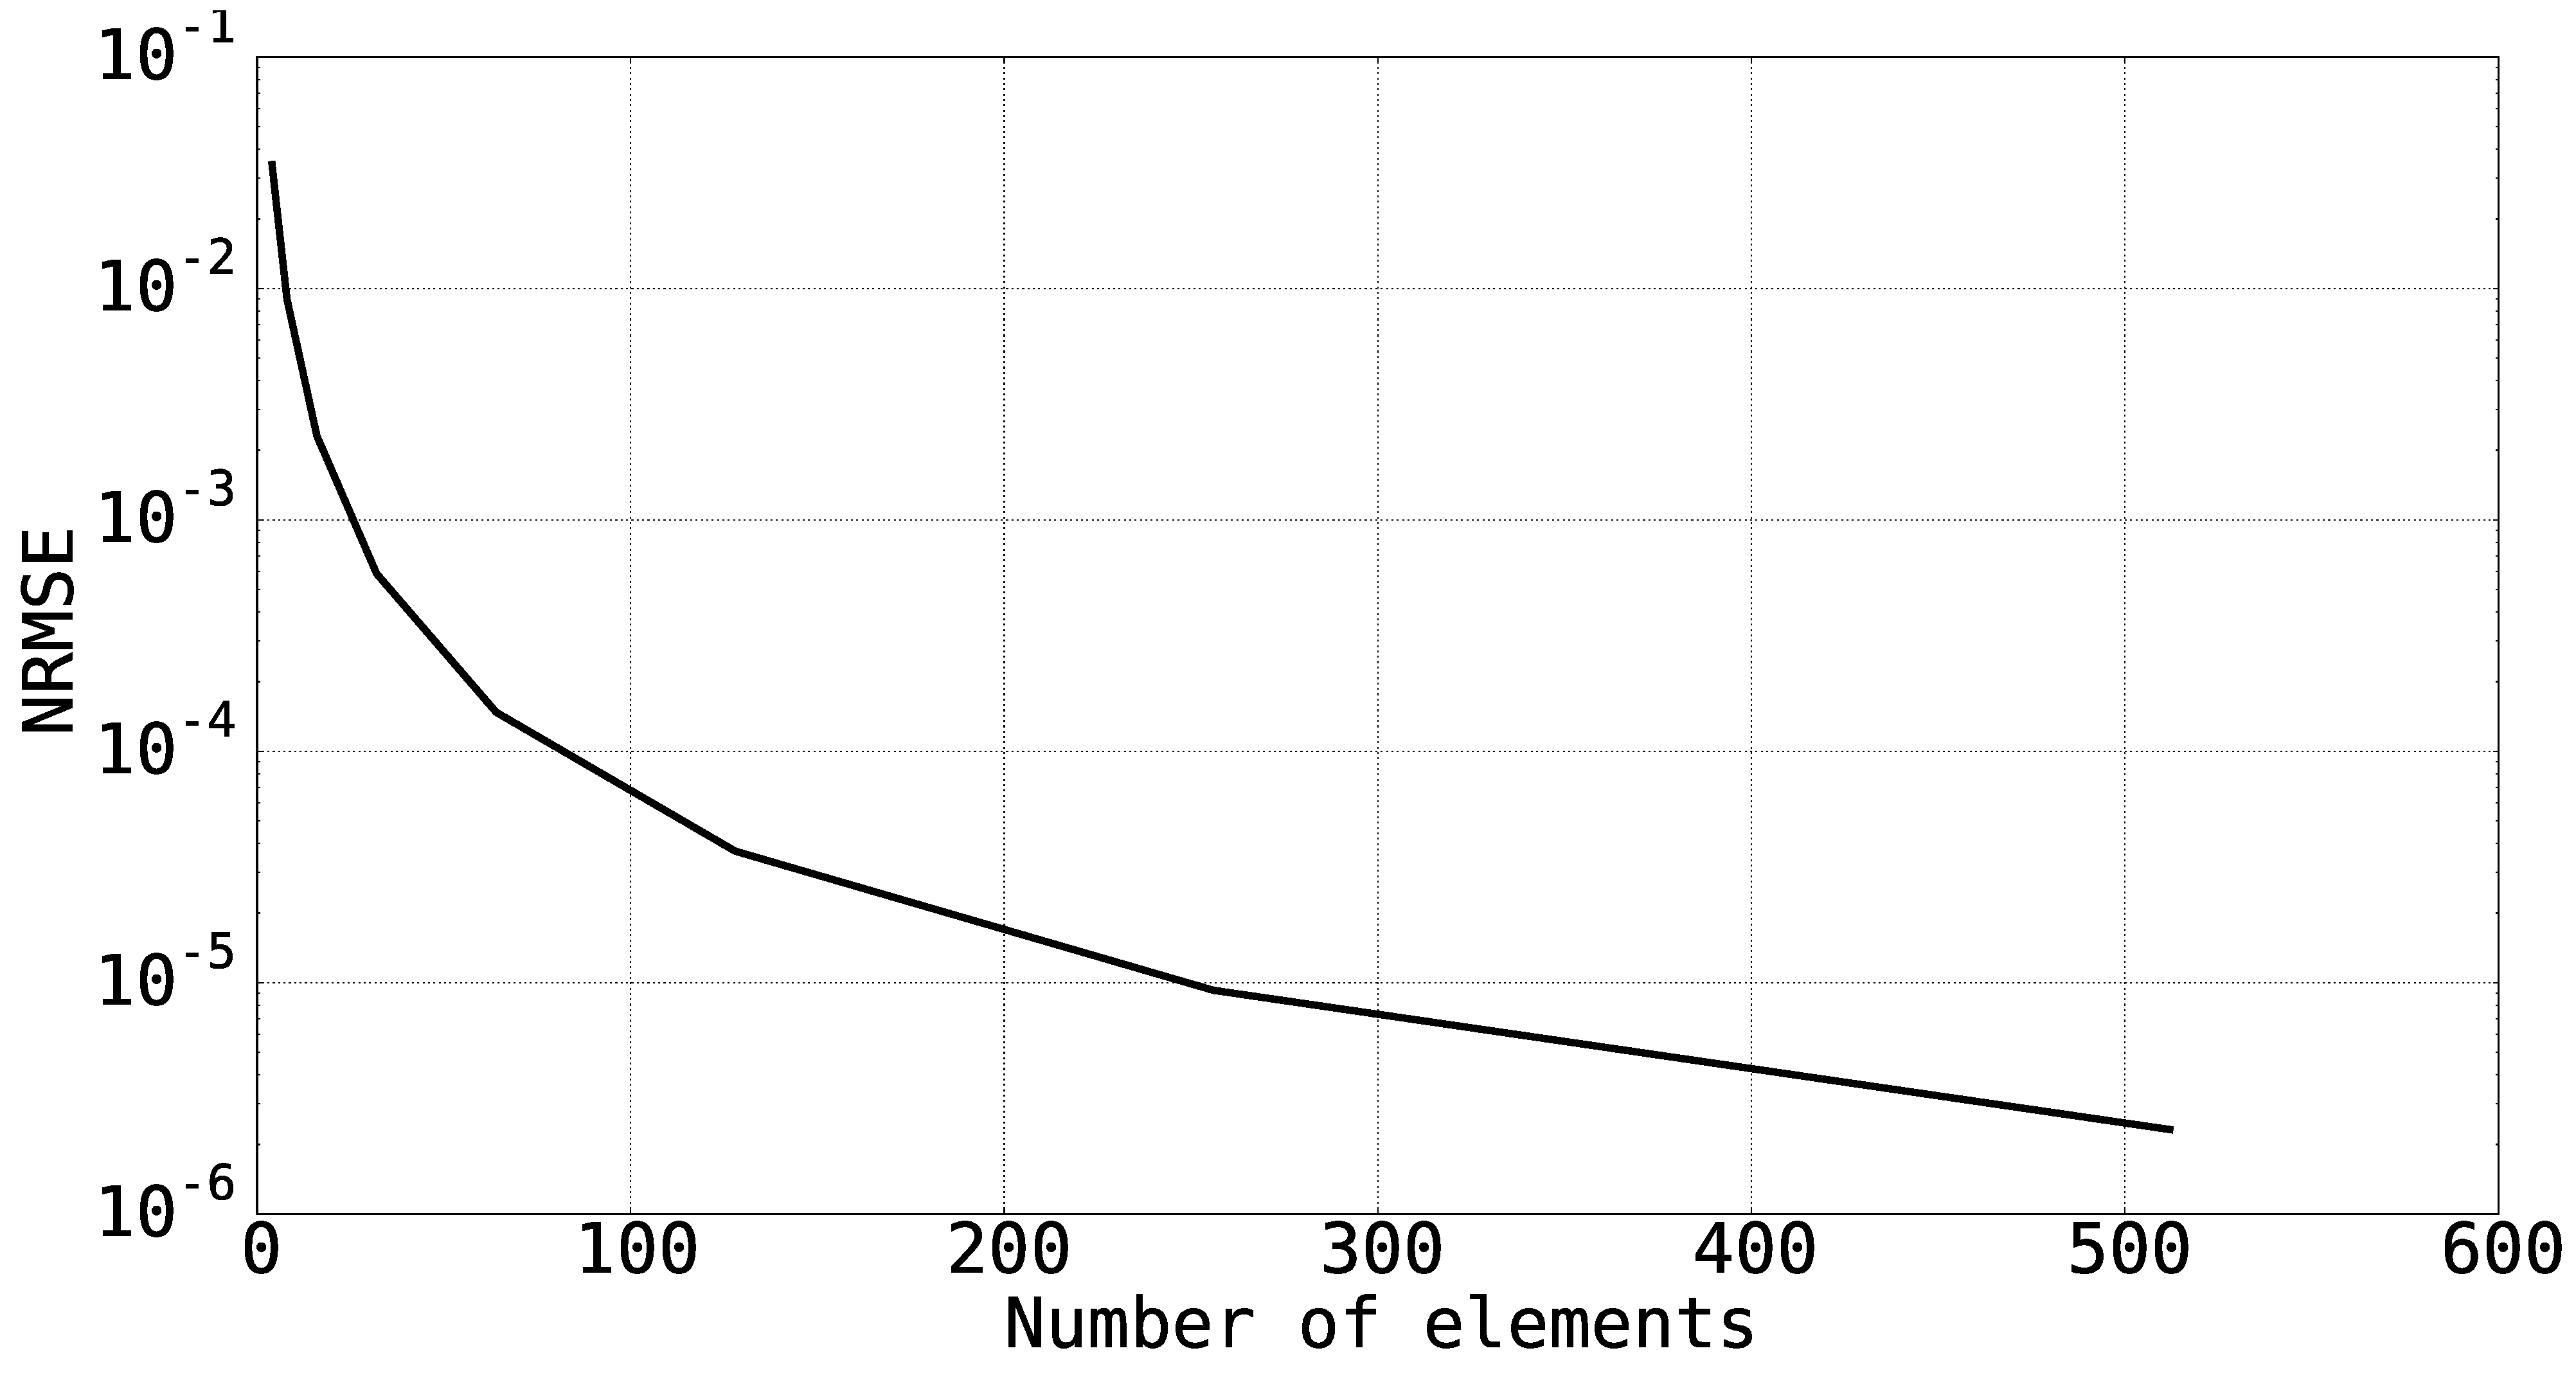
\includegraphics[width=14.00cm]{Chapter_2/figure/axial_bar_governing_equation_mesh_convergence.eps}
    \caption{Mesh convergence of the finite elements analysis for axial bar.}
    \label{fig:C2_axialBarSolution}
\end{figure}

The discrete sensitivity equation is derived by differentiating Equation \eqref{eq:C2_discretizedBarEquation} with respect to the shape of the domain as shown in Equation \eqref{eq:C2_discretizedSAequation_beforeSimplification}.

\begin{equation}\label{eq:C2_discretizedSAequation_beforeSimplification}
    \left[ \frac{\partial K}{\partial b} - \frac{\partial K_s}{\partial b} \right] [U] + 
    [K - K_s] \left[ \frac{\partial U}{\partial b} \right] = 
    \left[ \frac{\partial F_d}{\partial b} \right] - 
    \left[ \frac{\partial F_p}{\partial b} \right]
\end{equation}

Where $b$ is the design variable. $[K_s]$ is not affected by the design variable; therefore, its derivative with respect to $b$ is equal to zero. The same argument can be made for the point load $F_p$. Using these observations, Equation \eqref{eq:C2_discretizedSAequation_beforeSimplification} is simplified as:

\begin{equation}\label{eq:C2_discretizedSensitivityEquation}
    \left[ \frac{\partial U}{\partial b} \right] = 
    [K - K_s]^{-1}
    \left\{
    \left[ \frac{\partial F_d}{\partial b} \right] - \left[ \frac{\partial K}{\partial b} \right] [U]
    \right\}
\end{equation}

In Equation \eqref{eq:C2_discretizedSensitivityEquation}, $[U]$ is known as the result of solving the governing equation \eqref{eq:C2_discretizedBarEquation}that change in and $\dfrac{\partial F_d}{\partial b}$ is easily calculated since the distributed force is analytically known. $\dfrac{\partial K}{\partial b}$ is calculated by differentiating Equation \eqref{eq:C2_stiffnessMatrixOfBar}. It should be noted that the change in bar length, $L$, only affects $l_3$. Therefore, $\dfrac{\partial l_3}{\partial L}$ is equal to one. Finally, the sensitivity of the stiffness matrix to the shape design variable for a simple case of Equation \eqref{eq:C2_stiffnessMatrixOfBar} is written as:

\begin{equation}\label{eq:C2_sensitivityOfStiffnessMatrixOfBar}
    \left[ \frac{\partial K}{\partial L} \right] = 
    -EA
    \begin{bmatrix}
    0 & 0 & 0 & 0 \\
    0 & 0 & 0 & 0 \\
    0 & 0 & 1/l_3^2 & -1/l_3^2 \\
    0 & 0 & -1/l_3^2 & 1/l_3^2
    \end{bmatrix}
\end{equation}

The sensitivity results of solving the discrete Equation \eqref{eq:C2_discretizedSensitivityEquation} are compared with the analytical result from Equation \eqref{eq:C2_axialBarSensitivitySolution}. This comparison is shown as NRMSE values in Figure \ref{fig:C2_barDiscreteSensitivityAnalysis}. As shown here, the analytical and discrete sensitivity results agree very well. Moreover, the error decreases as we increase the number of elements.

\begin{figure}[h]
    \centering
    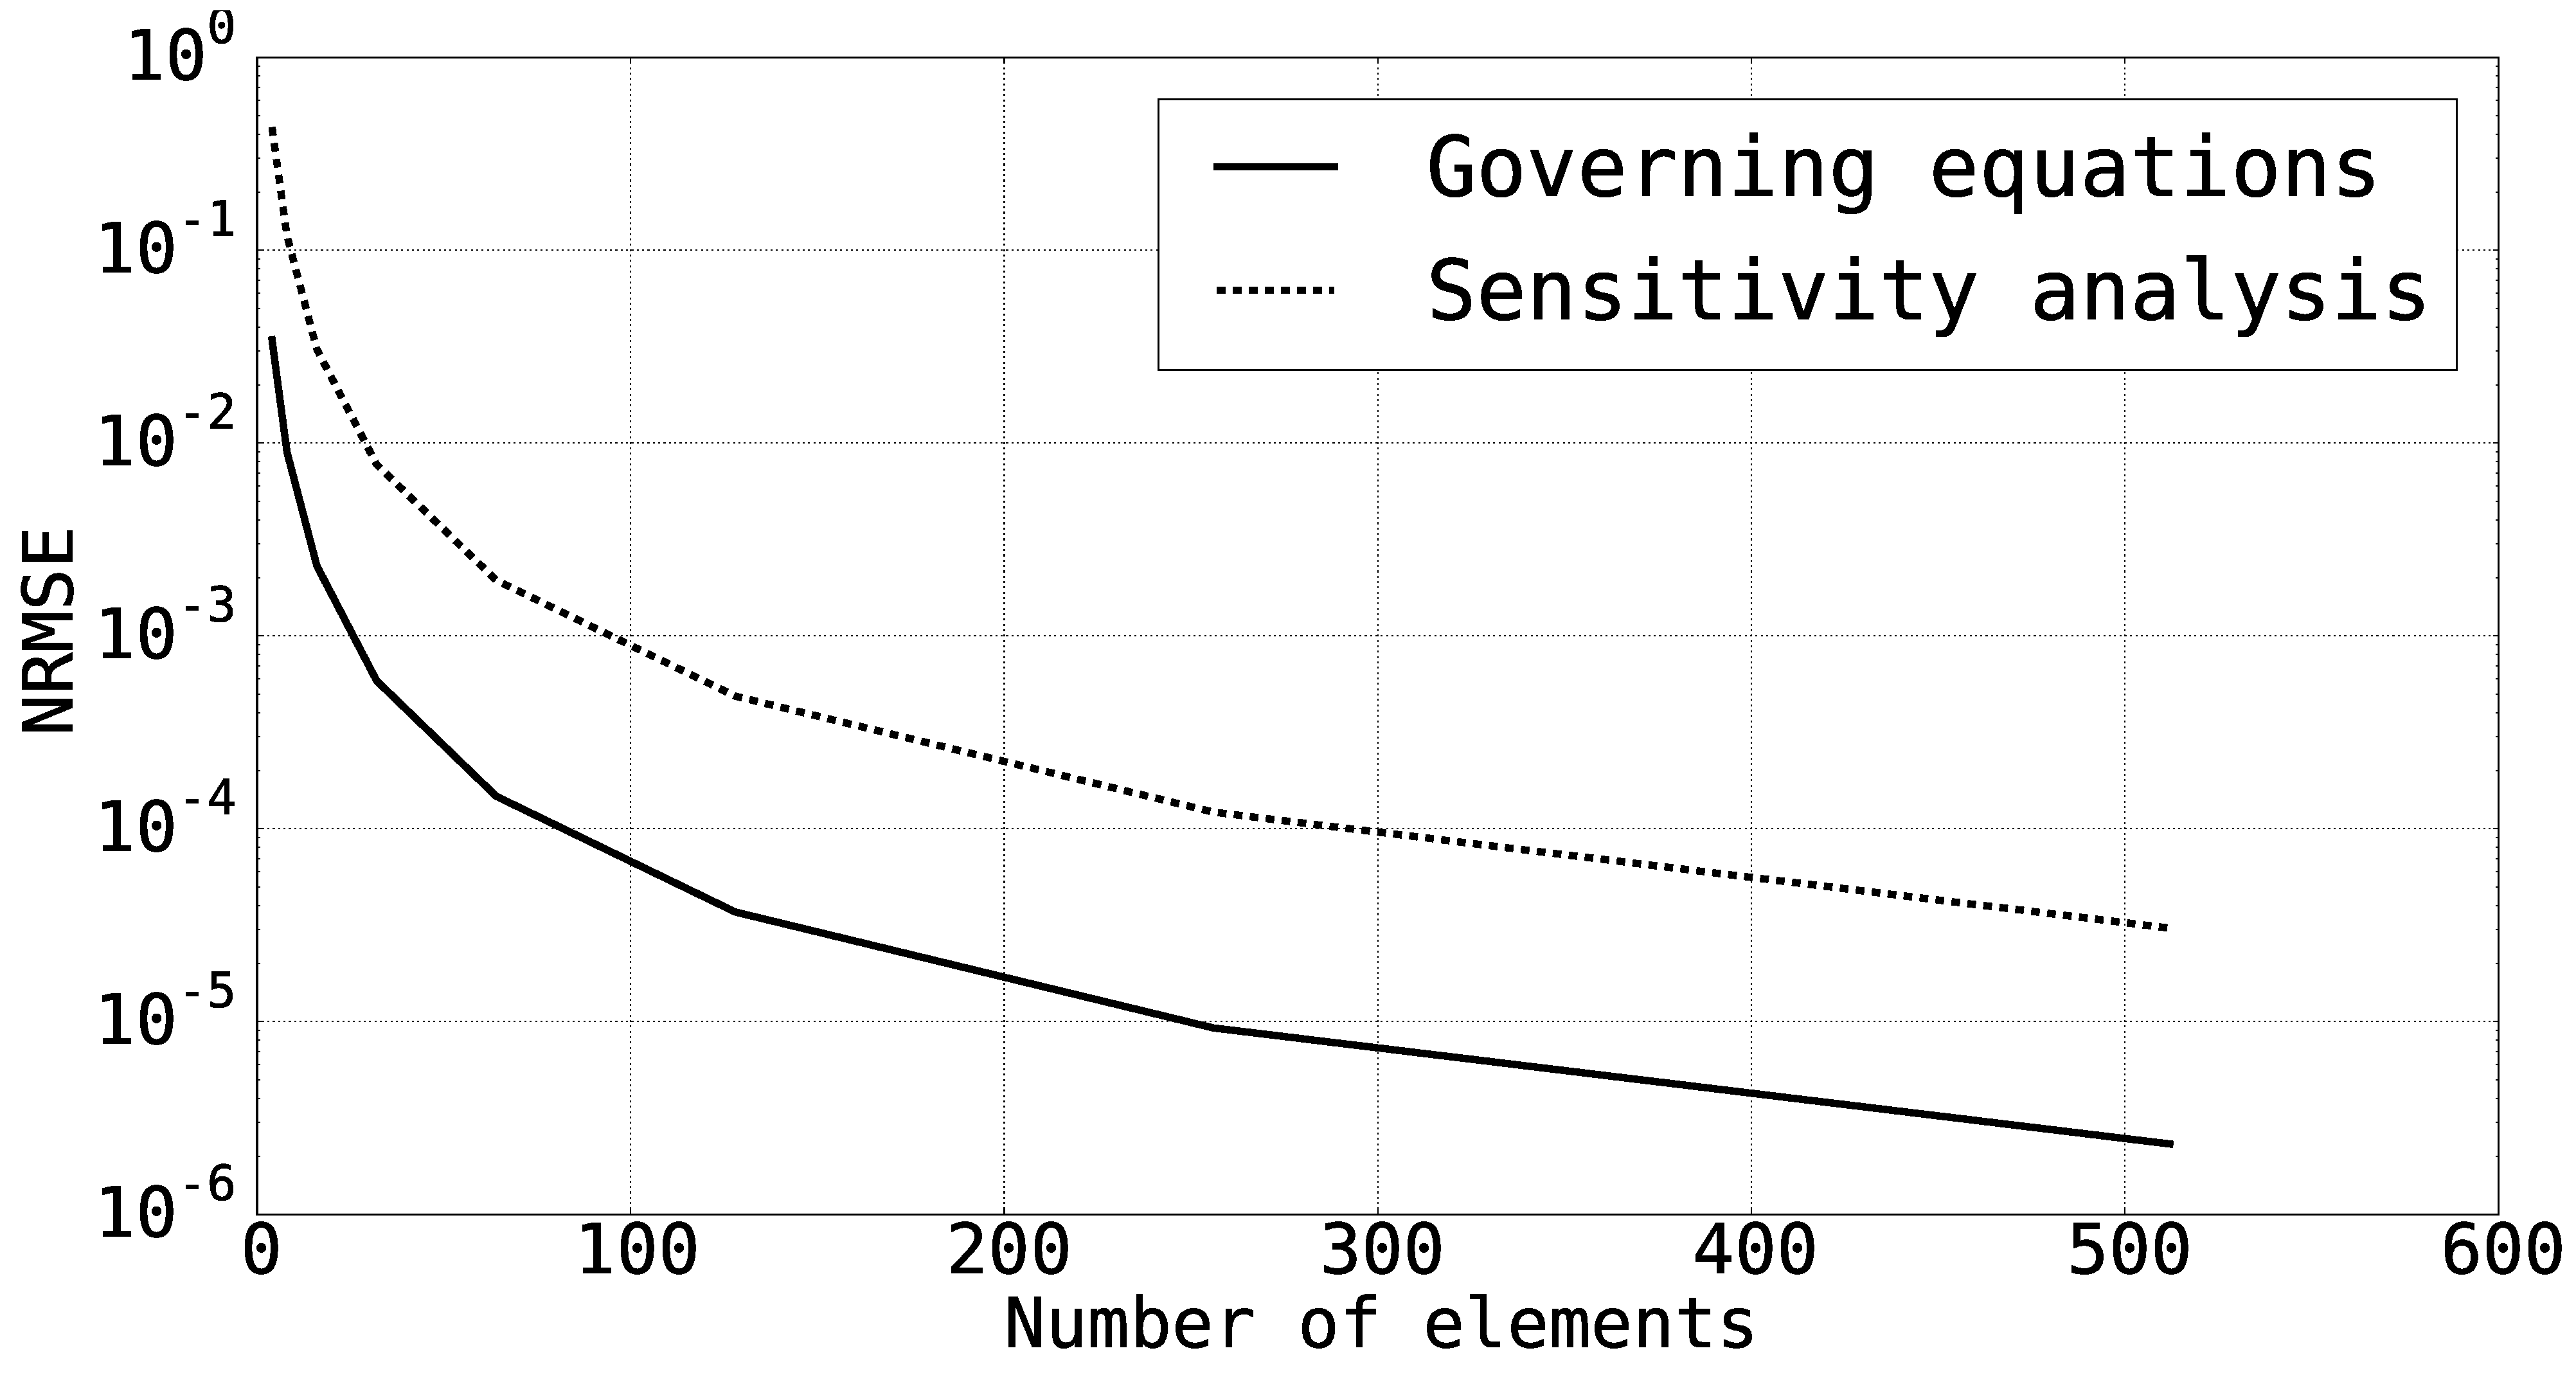
\includegraphics[width=14.00cm]{Chapter_2/figure/axial_bar_discrete_sensitivity_analysis.eps}
    \caption{Mesh convergence of the discrete sensitivity analysis for the axial bar.}
    \label{fig:C2_barDiscreteSensitivityAnalysis}
\end{figure}
% ======================================================================================
\input{Chapter_2/Chapter_2_Continuum_Sensitivity_Formulation.tex}
% ======================================================================================
\section{Summary}
In summary, we looked at two main approaches used to calculate the sensitivity response of a system. The discrete method is based on differentiating the discretized governing equations whereas in continuum method the governing equation are differentiated first and then discretized. We applied these techniques to a simple 1-D heat transfer problem and calculated the sensitivity of response to shape design parameter. The sensitivities are calculated in the local form for each of these methods and compared with the analytical results where they show good comparison. It is showed that by using the continuum sensitivity analysis, the differential operators used in the solution of governing equations are reused in the sensitivity analysis. This effectively means that the black-box solver used in the simulation step can be reused with new boundary conditions for solving the sensitivity response. As showed in the example problem, this is not possible when using discrete method. This is mainly due to the fact that the discrete operators will be affected by differentiating the discretized governing equations with respect to design variables. Therefore, more details about the analysis needs to be known when using discrete approach compared to the continuum. Continuum sensitivity approach is used in this research due to its ability to treat the analysis as black-box for solving both the governing equations and the sensitivity response. However, the result of sensitivity analysis is still the local sensitivities which needs to be transformed to the total form using the chain rule. This is not favourable because it is another step on top of an already expensive analysis. We are proposing to use a non-body conformal approach such as immersed boundary method for analysis to remove this step from the sensitivity calculation.

\chapter{The Immersed Boundary Method}
Immersed boundary methods are class of techniques in computational fluid dynamics where the governing equations are solved on cartesian grid that does not conform to the shape of the body in the flow. This is opposed to well known body-conformal techniques where the computational mesh accurately represents the shape of the domain. The boundary condition on the immersed surfaces are not applied explicitly, instead an extra forcing function is added to the governing equations or the discrete numerical scheme is updated near the boundary. The immersed boundary technique is in special interest to us since it removes the mesh sensitivity calculation from the analysis. In this chapter we talk about different classes of immersed boundary technique and apply them to a simple problem. The applicability of these methods in the continuum sensitivity analysis is also discussed. At the end of this chapter, we will chose couple of immersed boundary techniques for sensitivity analysis implementation.

% ======================================================================================
\section{Introduction}
When people started to use computational models in the design of systems, it was usually sufficient to include single physics into the design. The simulations were usually based on structural solvers using finite elements analysis (FEA) or computational fluid dynamics (CFD) simulations. The design requirements for different systems has been drastically changed compared to the initial designs where these computational methods have been applied. The requirements such as higher fuel efficiency, improved controllability, higher stiffness to mass ratios and lower radar signature have forced the designers to develop more unconventional configurations. For example, on way to reduce the infra-red signature of the aircraft engine is to remove it from hanging underneath the wing and put it inside of the aircraft. However, by doing this as massive heat source will be added the structure. The thermal expansion due to this excessive heat load needs to be incorporated into the structural analysis of the system. It requires a multidisciplinary analysis combining thermal analysis for heat transfer and structural analysis for thermal expansion and other structural loads \cite{deaton2013stiffening}.

The multidisciplinary analysis is required for many engineering application however the one that is used most is the interaction of fluid and a deformable structure. This is commonly known as a Fluid-Solid Interaction (FSI) problem. Fluid–structure interaction (FSI) problems are dealt with in many different engineering applications, such as fluttering and buffeting of bridges \cite{jain1996coupled}, vibration of wind turbine blades \cite{arrigan2011control}, aeroelastic response of airplanes \cite{farhat2006provably}. FSI problems are also seen in blood flows in arteries and artificial heart valves \cite{sotiropoulos2009review}, flying and swimming \cite{kern2006simulations}. The conventional approach for simulating such problems is the Arbitrary Lagrangian–Eulerian (ALE) method. ALE methods are based on body- conforming grids to track the location of the fluid–structure interface. ALE methods have been applied to many FSI problems however, they are cumbersome if not impossible to apply to FSI problems with large deformations for complicated boundary shapes.

Immersed boundary (IB) methods are considered a separate family of methods used for modelling FSI problems with complicated boundary shapes and large deformations. IB methods, are based on solving the governing equations for fluids on a fixed grid. Although this computational grid can be structured (Cartesian) or unstructured, most methods are based on structured grid. When using structured grid, extremely efficient computational methods can be utilized on to solve the governing equations. The fluid–structure boundaries are represented by a set of independent nodes. The solid boundary effect on the flow is formulated either by introducing fictitious body forces in the governing equations or by locally modifying the structure of the background grid.

IB has several advantages over the ALE methods. Probably the biggest advantage is the simplification of the task of grid generation. Generating body-conformal grid for a complex shape is usually very complicated. The objective is to construct a grid that provides adequate local resolution with the minimum number of total grid points.  This requires a significant input from the user and is an iterative process. For complicated boundaries the unstructured grid approach is better suited however the grid quality is reduced for extremely complicated geometry. In contrast, for a simulation carried using an IB method, grid complexity and quality are not affected by the complexity of the geometry. 

This advantage becomes even more clear for flows with moving boundaries. The ALE approach requires generating a new mesh or deforming the old mesh to match the new boundary shape at each time step. The solution from last time step is also required to be projected to this new computational mesh. Both of the deformation/projection can affect the accuracy, robustness and the computational cost associated the the simulation. On the other hand, the boundary motion in IB method can be handled with rather ease because the computational mesh does not depend on the shape of the boundary. Therefore, although a significant progress in simulating flows using ALE methods has been made in the recent years \cite{lomtev1999discontinuous, farhat2004cfd, cheng2005fluid}, the IB method still remains an attractive alternative for such problems due to its simplicity and cost.

In the following sections of this chapter we first look at the governing equations for the fluid and solid domain. Followed by this different approaches for modelling the follow using IB method are discussed in detail. We apply different IB techniques to a simplified problem to compare the efficiency and simplicity of implimentation. The results are compared with body-conformal solution approach for accuracy comparison. Finally we assess different IB methods with regards to their applicability of the Continuum Sensitivity Analysis (CSA) framework.

% ======================================================================================
\section{Governing Equations}
In the fluid region $\Omega_f$, the governing equations for incompressible flow of a Newtonian fluid are known as Navier-Stokes (NS) equations. In the compact indicial notation, the NS equations are written as

\begin{subequations}\label{eq:C3_GE}
\begin{equation}\label{eq:C3_continuity}
	\frac{\partial u_i}{\partial x_i} = 0
\end{equation}
\begin{equation}\label{eq:C3_momentum}
	\frac{\partial u_i}{\partial t} + \frac{\partial u_i u_j}{\partial x_j} = 
	-\frac{1}{\rho_f	} \frac{\partial p}{\partial x_i} + 
	\nu \frac{\partial}{\partial x_j} \left( \frac{\partial u_i}{\partial x_j} \right) + 
	f_i
\end{equation}
\end{subequations}

where the repeated indices imply summation and $i,j=1,2,3$. $x_i$ are the spatial coordinates, $u_i$ are the velocity components of the fluid in $i$ direction, $\rho_f$ is the fluids density, $p$ is the pressure, $\nu$ is the kinematic viscosity, and $f_i$ are body forces. These forces are used in the IB technique to represent the effect of immersed boundaries on the fluid. In general purpose CFD solvers, due to the use of unstructured grid to represent the shape, it is usually required to use mappings (Jacobian) to convert the physical coordinate the a computational coordinate. This will become problematic when we have skewed elements with cause the mapping become singular. This step is removed in the IB approach since the governing equations \eqref{eq:C3_GE} are discretized on a Cartesian  grid.

The solid domain is modelled using linear elastic theory in this work. The governing equations are written as

\begin{subequations}\label{eq:C3_linearEalsticityEquations}
\begin{equation}
	\sigma_{ji,j} + F_i = \rho_s \partial_{tt} u_i
\end{equation}
\begin{equation}
	\epsilon_{ij} = \frac{1}{2} \left( u_{j,i} + u_{i,j} \right)
\end{equation}
\begin{equation}
	\sigma_{ij} = C_{ijkl} \epsilon_{kl}
\end{equation}
\end{subequations}

where $\sigma$ is the Cauchy stress tensor, $\epsilon$ is the strain tensor, $u$ is the displacement vector, $C$ is stiffness tensor, $F$ is the body force, and $\rho_s$ is the mass density of solid. These governing equations are solved to track the motion of of the solid boundary. 

To solve the coupled system of equations of \eqref{eq:C3_GE} and \eqref{eq:C3_linearEalsticityEquations} we need to have boundary conditions. The boundary conditions of \eqref{eq:C3_GE} are defined as pressure or velocity magnitudes on the outer boundaries of the domain. After solving Equation \eqref{eq:C3_GE}, the loads on the structure can be calculated by integrating the pressure from the fluid solid over the solid boundaries. This will be the boundary load used for solving Equation \eqref{eq:C3_linearEalsticityEquations}. When the governing equation for the solid region is solved, the displacement of the solid domain is known. This is fed into the CFD solver to update the solid boundary location for fluid domain. This will change the solution of fluid's solver resulting in different pressure distribution. This process is repeated until a convergence is satisfied. The convergence can be defined as change in the structure deflection for two subsequent steps for a static problem.

% ======================================================================================
\section{Benchmark Case}
We define a 1D benchmark problem to investigate different IB formulations in detail. In one dimensional space the equations of incompressible flow are not very interesting and it is not simple to write a one-dimensional analogue of the IB to capture all of its features. However, for a simple one dimensional problem we can understand different formulations of IB method and later apply it to higher dimensions. Moreover, for the sake of sensitivity analysis better understanding of the problem can be achieved for a simplified model. The other reason for working with a simplified model is the availability of analytical results that can be used for verifying the results we get from the numerical solvers. As the final note, for this benchmark case we mainly focused on the fluid domain, the structures can be easily added to this formulation.

To derive the one dimensional benchmark case we start with the Navier-Stokes equations. Consider a viscous incompressible fluid in the channel $0 \geq y \leq 1$, $-\infty < x < \infty$ as shown in Figure \ref{fig:C3_benchmarkCase}.

\begin{figure}[h]
	\centering
	\includegraphics[width=14.00cm]{Chapter_3/figure/C3_infinite_channel.png}
	\caption{1D benchmark case for IB method.}
	\label{fig:C3_benchmarkCase}
\end{figure}

We can also assume that the boundary conditions are periodic in $x$. Next suppose that there is a horizontal plate running through the length of this channel at $y=y_0$ and moving with $u_0$ velocity in horizontal direction. We assume no-slip condition where the fluid and the plate meet. This will force the fluid to accelerate in $x$ direction due to the viscous stress from the moving plate. We expect no motion in $y$ direction and can drop all terms in the NS equations containing $u_j$ velocity. Due to the continuity equation \eqref{eq:C3_continuity}, there is no variation in the $x$ direction so we can drop all the terms that involve with $x$ variation as well. This enables us to simplify the NS equation of \eqref{eq:C3_momentum} into Equation \eqref{eq:C3_benchmarkProblem}. It should be noted that the continuum equation \eqref{eq:C3_continuity} is automatically satisfied.

\begin{subequations}\label{eq:C3_benchmarkProblem}
\begin{equation}
	u_t = \mu u_{yy} \quad \text{in } \Omega_f
\end{equation}
\begin{equation}
\begin{cases}
	u = u_0 \quad \text{at } y = 1 \\
	u = 0 \quad \text{at } y = 0
\end{cases}
\end{equation}
\end{subequations}

Equation \eqref{eq:C3_benchmarkProblem} is transient in nature however, its steady state solution can be calculated by setting the time derivative equal to zero. This equation governs what is commonly known as Couette flow in introductory courses in fluid dynamics. The analytical solution for this equation is shown in Equation \eqref{eq:C3_benchmarkAnalyticalSolution}.

\begin{equation}\label{eq:C3_benchmarkAnalyticalSolution}
	u = u_0 x
\end{equation}

We will use this analytical solution to verify the result of the different IB methods defined in the following sections.

% ======================================================================================
\section{Immersed Boundary Classification}
In general, IB methods can be classified in three main families: i) discrete forcing, ii) continuum forcing, and iii) cut-cell methods. This classification is based on how the interface conditions are handled in the IB algorithm. In this section we present the essence of each method and try to point their primary advantages and disadvantages. Moreover, each of the discussed IB techniques will be applied to the benchmark problem where the results are verified with the analytical solution. In general, the immersed boundary approach is based on modifying the NS equations for imposing the boundary conditions. This modification can be done in three different ways that leads to a fundamental dichotomy in IB method.

\subsection{Discrete Forcing Method}

\subsubsection{Formulation}
\subsubsection{Implimentation for Couette Flow Problem}
\subsection{Continuum Forcing Method}
In this implementation of the immersed boundary, a forcing equation is added to the continuous governing equation \eqref{eq:C3_momentum} to represent the effect of the boundary. The continuous IB technique is the original method developed by Peskin \cite{peskin1972flow} for coupled simulation of blood flow due to the contraction of heart muscle. In this approach, the immersed boundary is represented by a set of elastic fibers that their locations are tracked in a Lagrangian fashion by a collection of massless points. These points move with the local fluid velocity. Therefore, the location of the $k$-th Lagrangian point, $X_k$ is governed by the following equation

\begin{equation}
	\frac{\partial X_k}{\partial t} = u(X_k, t)
\end{equation}

where $u$ is the velocity of the fluid at location $X_k$. The location of fluid nodes, $x$, does not necessary coincide with the location of the Lagrangian points. Thus, it is required to map the velocities from the Eulerian domain, where the fluid's equation of motion are solved, to Lagrangian nodes. In a purely continuum problem, this can be done using the Dirac delta functions. The property of the Dirac delta function that enables the mapping between the Euler and Lagrangian domain is shown in the following equation

\begin{equation}
	\int_{\Omega_f} f(x) \delta(x - X_k) = f(X_k)
\end{equation}

As can be seen here, by convoluting the function of interest and the delta function, we can evaluate our function of interest at any location where the delta function is defined. By defining the delta function at $X_k$ and using velocity from CFD solver as function $f$, we can evaluate the needed velocity for IB at any arbitrary point $X_k$. Although this is the main idea of mapping data to Lagrangian domain, this approach becomes unstable in practice \cite{lee2003stability}. In the practical implementation of immersed boundary method, the effect of delta function need to be expanded to couple of nodes around $X_k$. This is achieved by relaxing the delta function. The relaxed delta function is generally refereed to as regularized delta function \cite{shin2008assessment}. The reqularized delta functions of Equation \eqref{eq:C3_regularizedDeltaFunctions} are ploted in Figure \ref{fig:C3_regularizedDeltaFunctions}.

%\subsubsection{Formulation}
%\subsubsection{Implimentation for Couette Flow Problem}
%\subsection{Cut-cell Method}
%\subsubsection{Formulation}
%\subsubsection{Implimentation for Couette Flow Problem}
%\section{Application in Continuum Sensitivity Analysis}
%\section{Summary}
\chapter{Shape Sensitivity Analysis for Immersed Boundary Method}

% ======================================================================================
\section{Introduction}
\section{Sensitivity Problem Formulation}
\subsection{Regularized Delta/Heaviside Function}
\subsection{Direct Method}
\subsection{Adjoint Method}
\section{Shape Sensitivity of Flow over Cylinder}
\section{Shape Sensitivity of Flow through Nozzle}
\section{Summary}
\chapter{Shape Sensitivity Analysis for Coupled FSI Problem}

% ======================================================================================
\section{Problem definition}
\subsection{Governing Equations}
\subsection{FSI Coupling}
\section{Results}
\section{Summary}

\chapter{Future work}

% ======================================================================================
\section{Level set method}
\section{Dynamic Aeroelastic Coupling}
%
%-----------------------------------------------------------------------
% Bibliography
%-----------------------------------------------------------------------
\clearpage \phantomsection %used to correctly anchor hyperlinks
\renewcommand\baselinestretch{1.5}
\addcontentsline{toc}{chapter}{Bibliography}
\bibliographystyle{aiaa}
\bibliography{Chapter_1/Chapter1Ref,Chapter_2/Chapter2Ref,Chapter_3/Chapter3Ref,Chapter_4/Chapter4Ref,Chapter_5/Chapter5Ref}
%
%-----------------------------------------------------------------------
% Appendices
%-----------------------------------------------------------------------
%%%%%%%%%%%%%%%%%%%
%\begin{appendices}
%\phantomsection %use \phantomsection command to correctly anchor hyperlinks
%\chapter[An Example Appendix]{Appendix A\\An Example}
\label{chap:AppA}
Here is an appendix\ldots not too difficult.
%\phantomsection
%\chapter[Another Example Appendix]{Appendix B\\Another Example}
\label{chap:AppB}
Again\ldots not too difficult.
%\end{appendices}
%%%%%%%%%%%%%%%%%%%
%
%
%
% End of document
\end{document} 
